\documentclass[fsharpNotes.tex]{subfiles}
\graphicspath{ {./figures/} }

\begin{document}
\chapter{Graphical User Interfaces}
\label{chap:windows}

A \idx{graphical user interface} (\idx{GUI}) uses graphical elements such as windows, icons, and sound to communicate with the user, and a typical way to activate these elements is through a pointing device such as the mouse or by touch. Some of these elements may themselves be textual, and thus most operating systems offer access to a \idx{command-line interface} (\idx{CLI}) in a window alongside other interface types.

An example of a graphical user interface is a web-browser, shown in \Cref{fig:safariGui}.
\begin{figure}
  \centering
  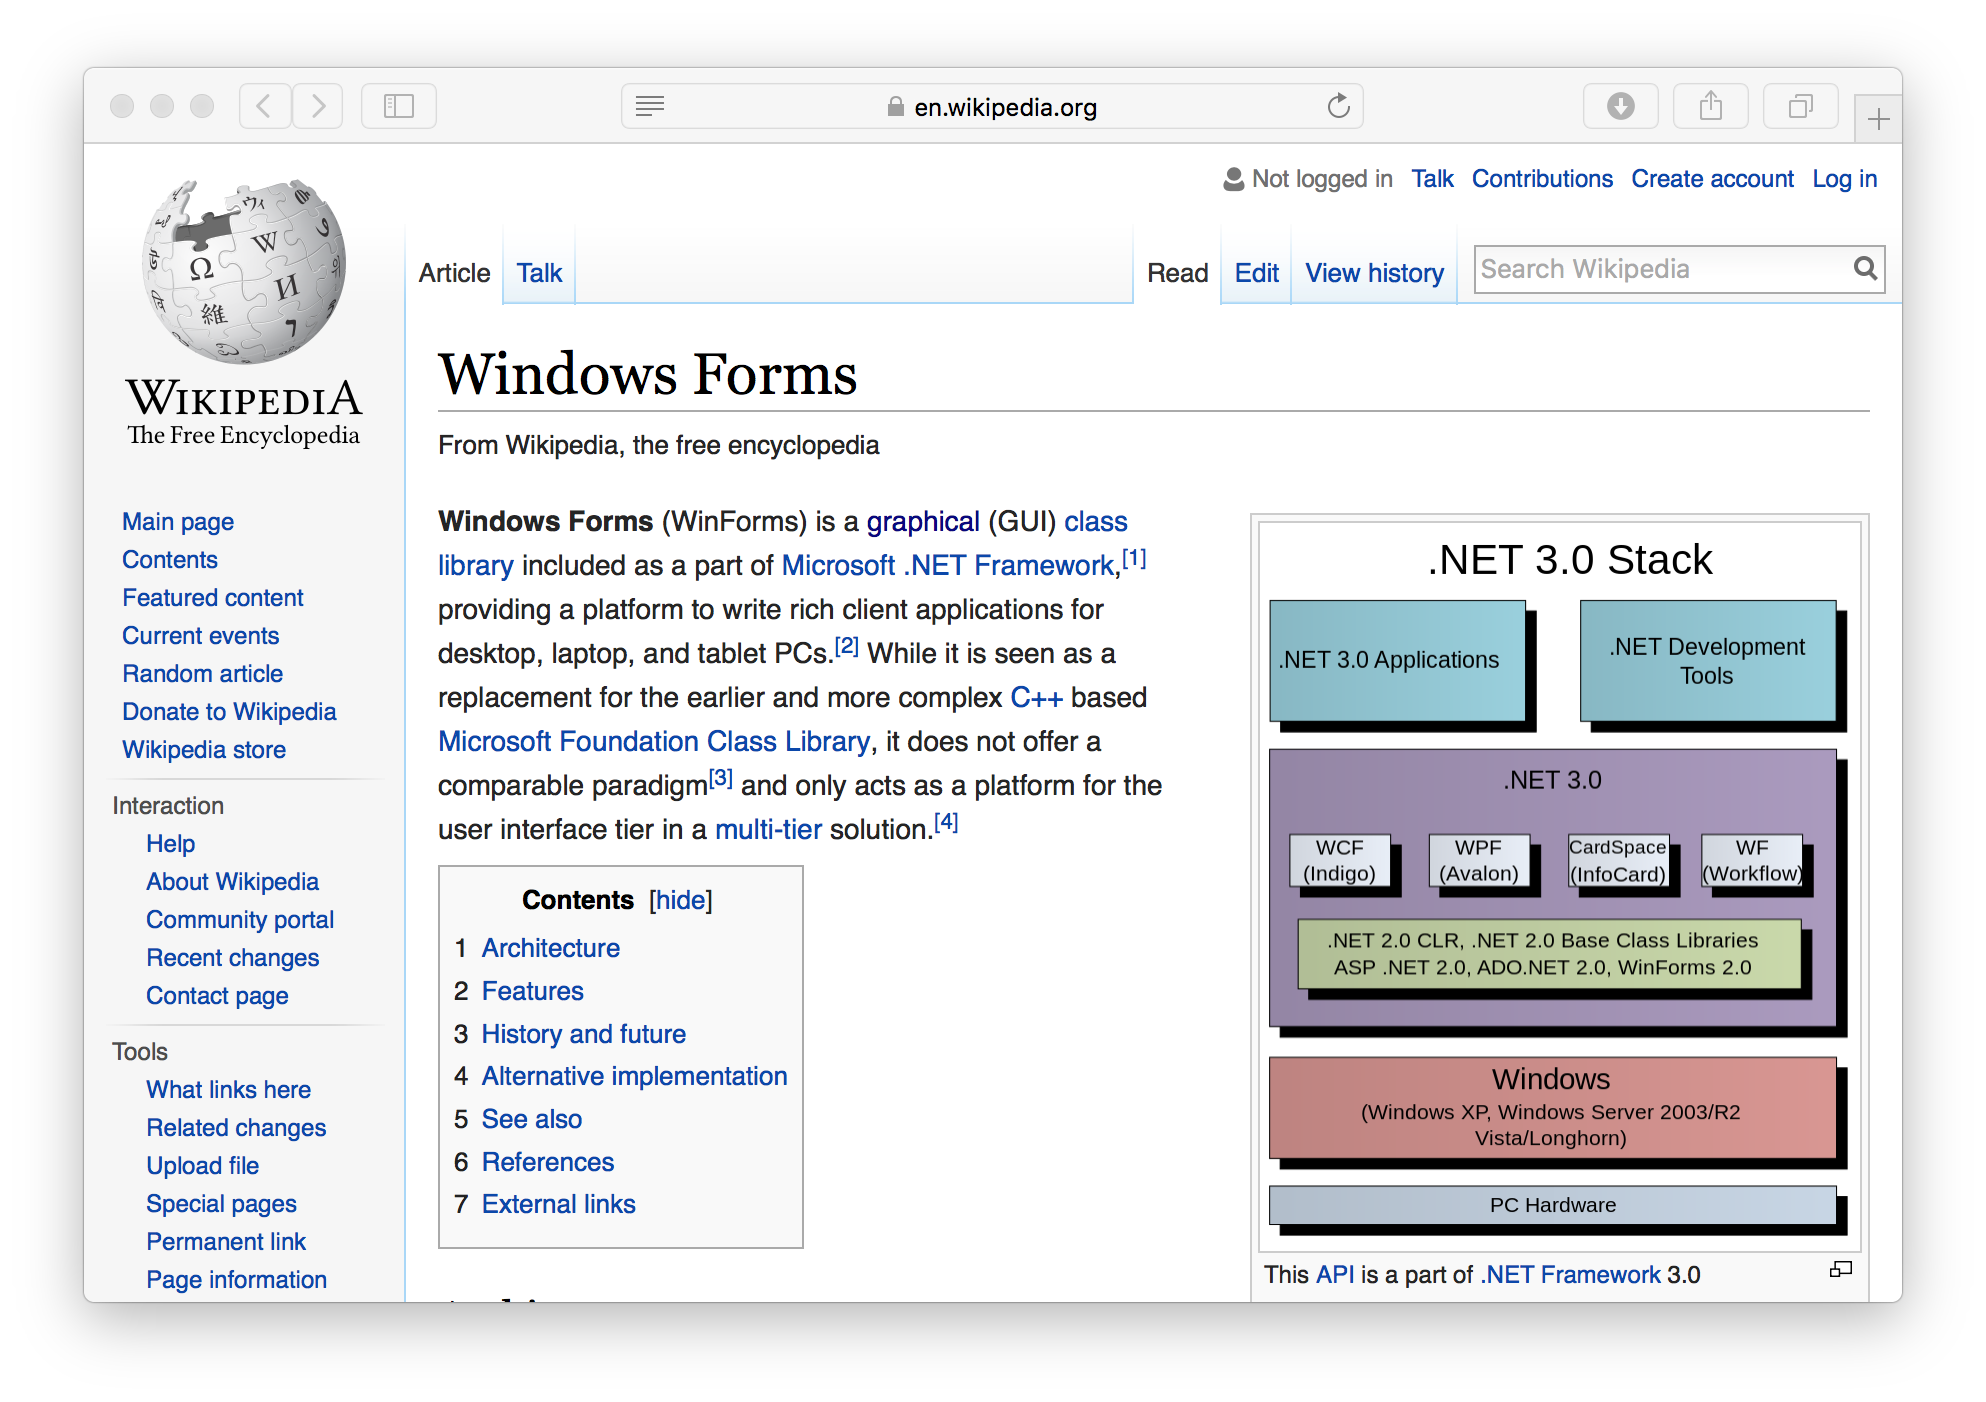
\includegraphics[width=0.8\textwidth]{safariWinForms}
  \caption{A web-browser is a graphical user interface for accessing a web-server and interacting with its services. Here the browser is showing the page \url{https://en.wikipedia.org/wiki/Windows_Forms} at time of writing.}
  \label{fig:safariGui}
\end{figure}
The program presents information to the user in terms of text and images, has active areas that may be activated by clicking, allows the user to go other web-pages by typing a URL or following hyperlinks, and can generate new pages through search queries.

F\# includes a number of implementations of graphical user interfaces, and at time of writing, both \idx{GTK+} and \idx{WinForms 2.0} are supported on both the Microsoft .Net and the Mono platform. WinForms can be used without extra libraries during compilation, and therefore will be the subject of the following chapter.

WinForms is a set of libraries that simplifies many common tasks for applications, and in this chapter, we will focus on the graphical user interface part of WinForms. A \idx{form} is a visual interface used to communicate information with the user, typically a window. Communication is done through \idx[control]{controls}, which are elements that display information or accept input. Examples of controls are a box with text, a button, and a menu. When the user gives input to a control element, this generates an \idx{event} which you can write code to react to. WinForms is designed for \idx{event-driven programming}, meaning that at runtime, most time is spent on waiting for the user to give input. See \Cref{chap:eventDriven} for more on event-driven programming.

Designing easy-to-use graphical user interfaces is a challenging task. This chapter will focus on examples of basic graphical elements and how to program these in WinForms.

\section{Opening a Window}
The namespaces \idx[System.Windows.Forms@\lstinline{System.Windows.Forms}]{\lstinline{System.Windows.Forms}} and \idx[System.Drawing@\lstinline{System.Drawing}]{\lstinline{System.Drawing}} are central for programming graphical user interfaces with WinForms. \lstinline{System.Windows.Forms} includes code for generating forms, controls, and handling events. \lstinline{System.Drawing} is used for low-level drawing, and it gives access to the \idx{Windows Graphics Device Interface} (\idx{GDI+}), which allows you to create and manipulate graphics objects targeting several platforms, such as screens and paper. All controls in \lstinline{System.Windows.Forms} in Mono are drawn using \lstinline{System.Drawing}. 

To display a graphical user interface on the screen, the first thing to do is open a window, which acts as a reserved screen-space for our output. In WinForms, windows are called forms. Code for opening a window is shown in \Cref{winforms/openWindow}, and the result is shown in \Cref{fig:openWindow}. Note that the present version of WinForms on MacOs only works with the 32-bit implementation of mono, \idx[mono32@\filename{mono32}]{\filename{mono32}}, as demonstrated in the example.
%
\fs{winforms/openWindow}{Create the window and turn over control to the operating system. See \Cref{fig:openWindow}.}
%
%
%\codeFromFile{winforms/openWindow}{openWindow}{Create the window and turn over control to the operating system.}
%
\begin{figure}
  \centering
  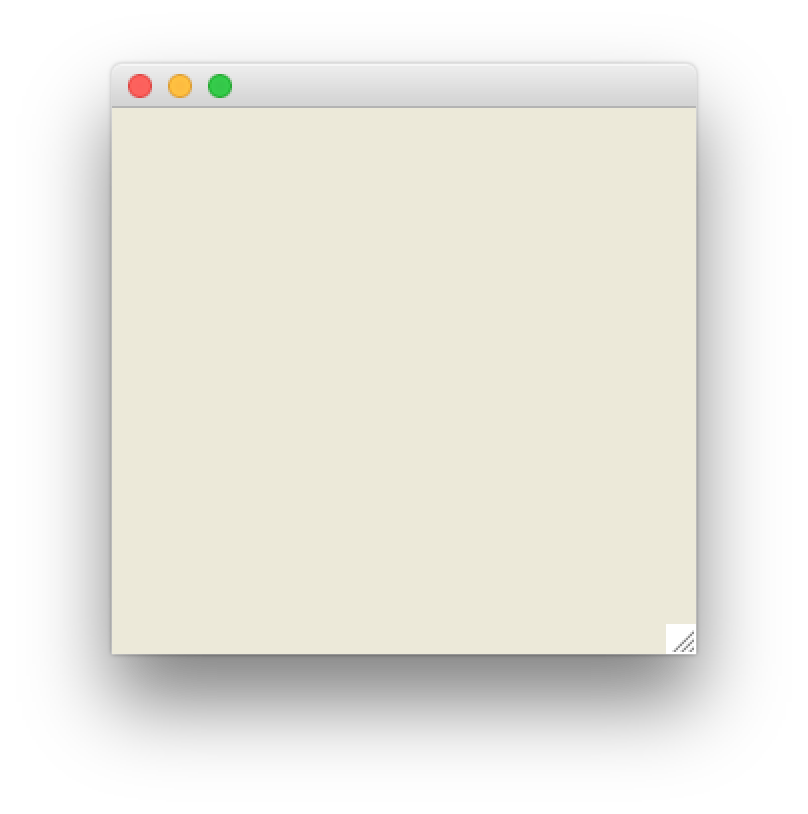
\includegraphics[scale=0.2]{openWindow}
  \caption{A window opened by \Cref{winforms/openWindow}.}
  \label{fig:openWindow}
\end{figure}
The \lstinline!new System.Windows.Forms.Form ()! creates an object (See \Cref{chap:oop}), but does not display the window on the screen. We use the optional \keyword{new} keyword, since the form is an \lstinline{IDisposable} object and may be implicitly disposed of. I.e., it is recommended to \advice{instantiate \lstinline{IDisposable} objects using \keyword{new} to contrast them with other object types.} Executing \lstinline!System.Windows.Forms.Application.Run! is applied to the object, then the control is handed over to the WinForms' \idx{event-loop}, which continues until the window is closed by, e.g., pressing the icon designated by the operating system. On the Mac OSX, that is the red button in the top left corner of the window frame, and on Window it is the cross on the top right corner of the window frame.

The window form has a long list of methods and properties. E.g., the background color may be set by \lstinline!BackColor!, the title of the window may be set by \lstinline!Text!, and you may get and set the size of the window with \lstinline!Size!. This is demonstrated in \Cref{winforms/windowProperty}.
%
\fsCode{winforms/windowProperty}{winforms/windowProperty}{Create the window and change its properties. See \Cref{fig:windowProperty}}{}
%
\begin{figure}
  \centering
  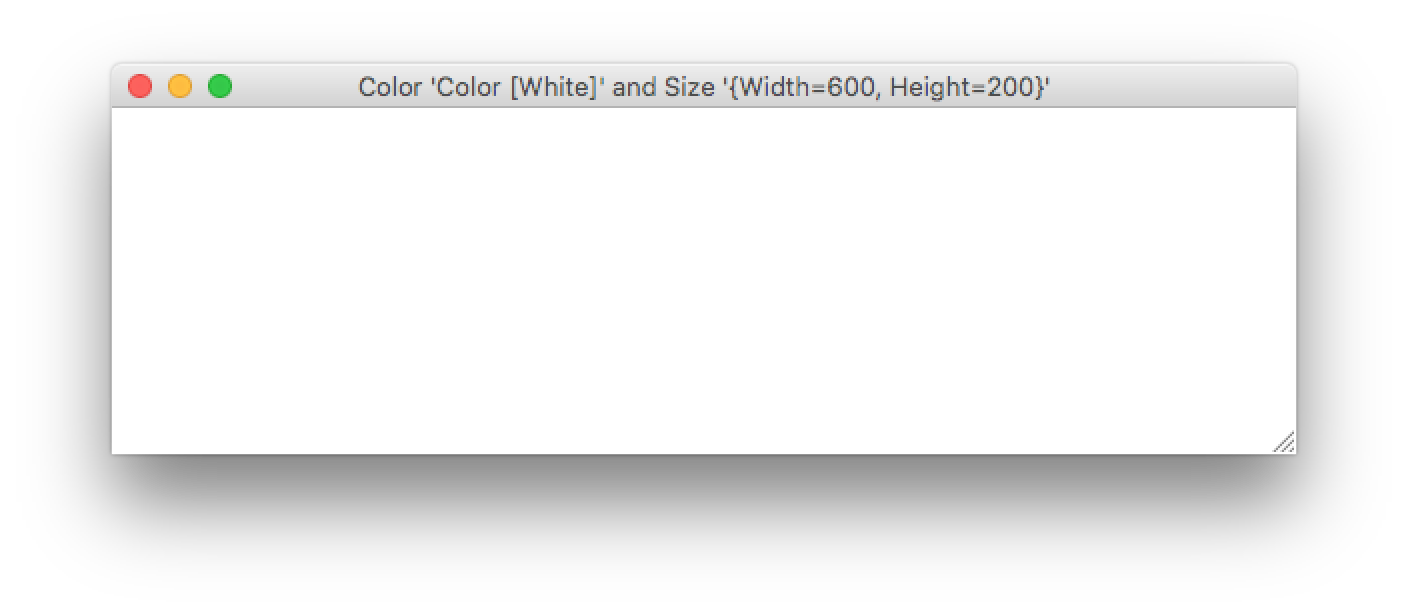
\includegraphics[scale=0.2]{windowProperty}
  \caption{A window with user-specified size and background color, see \Cref{winforms/windowProperty}.}
  \label{fig:windowProperty}
\end{figure}
%
These properties are \idx{accessors}, implying that they act as mutable variables. 

\section{Drawing Geometric Primitives}
The \idx[Color@\lstinline{Color}]{\lstinline{System.Drawing.Color}} is a structure for specifying colors as 4 channels: alpha, red, green, and blue. Some methods and properties for the Color structure is shown in \Cref{tab:color}.
\begin{table}
  \begin{center}
  \rowcolors{2}{oddRowColor}{evenRowColor}
  \begin{tabularx}{\linewidth}{|>{\hsize=1.15\hsize}X|>{\hsize=.85\hsize}X|}
    \hline
    \rowcolor{headerRowColor}  Method/Property & Description\\
    \hline
    \rowcolor{subHeaderRowColor} \multicolumn{2}{|>{\hsize=\dimexpr2\hsize+2\tabcolsep+\arrayrulewidth\relax}X|}{Properties of an existing color structure}\\
    \hline \lstinline{A : byte}
    &The value of the alpha channel.\\
    \lstinline{R : byte}
    &The value of the red channel.\\
    \lstinline{G : byte}
    &The value of the green channel.\\
    \lstinline{B : byte}
    &The value of the blue channel.\\
      \lstinline{ToArgb : unit -> int}
      &The 32-bit integer value of the color.\\
    \hline
    \rowcolor{subHeaderRowColor} \multicolumn{2}{|>{\hsize=\dimexpr2\hsize+2\tabcolsep+\arrayrulewidth\relax}X|}{Static properties returning a color structure by its name.}\\
    \hline \lstinline{Black : Color}
    &The ARGB value \lstinline{0xFF000000}.\\
    \lstinline{Blue : Color}
    &The ARGB value \lstinline{0xFF0000FF}.\\
    \lstinline{Brown : Color}
    &The ARGB value \lstinline{0xFFA52A2A}.\\
    \lstinline{Gray : Color}
    &The ARGB value \lstinline{0xFF808080}.\\
    \lstinline{Green : Color}
    &The ARGB value \lstinline{0xFF00FF00}.\\
    \lstinline{Orange : Color}
    &The ARGB value \lstinline{0xFFFFA500}.\\
    \lstinline{Purple : Color}
    &The ARGB value \lstinline{0xFF800080}.\\
    \lstinline{Red : Color}
    &The ARGB value \lstinline{0xFFFF0000}.\\
    \lstinline{White : Color}
    &The ARGB value \lstinline{0xFFFFFFFF}.\\
    \lstinline{Yellow : Color}
    &The ARGB value \lstinline{0xFFFFFF00}.\\
    \hline \rowcolor{subHeaderRowColor} \multicolumn{2}{|>{\hsize=\dimexpr2\hsize+2\tabcolsep+\arrayrulewidth\relax}X|}{Static methods for converting between color structures and integers representations.}\\
    \hline
      \begin{minipage}[t]{1.15\linewidth}
        \lstinline{FromArgb :}\\
        \hspace*{5mm}\lstinline{r:int * g:int * b:int -> Color}
      \end{minipage}
      &Create a color structure from red, green, and blue values.\\
      \begin{minipage}[t]{1.15\linewidth}
        \lstinline{FromArgb :}\\
        \hspace*{5mm}\lstinline{a:int * r:int * g:int * b:int -> Color}
      \end{minipage}
      &Create a color structure from alpha, red, green, and blue values.\\
        \lstinline{FromArgb : argb:int -> Color}
      &Create a color structure from a single integer.\\
      \hline
    \end{tabularx}
  \end{center}
  \caption{Some methods and properties of the \lstinline{System.Drawing.Color}  structure.}
  \label{tab:color}
\end{table}
Each channel is an 8-bit unsigned integer. The alpha channel specifies the transparency of a color, where values 0--255 denote the range of fully transparent to fully opaque, and the remaining channels denote the amount of red, green, and blue, where 0 is none and 255 is full intensity. As a shorthand, colors are often referred to as a single 32-bit unsigned integer, whose bits are organized in groups of 8 bits as 0xAARRGGBB, where AA is the alpha channel's values 0x00--0xFF etc. Any color may be created using the \lstinline!FromArgb! method, e.g., an opaque red is given by \lstinline!System.Drawing.Color.FromArgb (255, 255, 0, 0)!. There are also many build-in colors, e.g., the same red color is also a known color and may be obtained as \lstinline!System.Drawing.Color.Red!. For a given color, the 4 alpha, red, green, and blue channels' values may be obtained as the \lstinline!A!, \lstinline!R!, \lstinline!G!, and \lstinline!B! members, see \Cref{drawingColors}
%
\fs{drawingColors}{Defining colors and accessing their values.}
%

The namespace \lstinline{System.Drawing} contains many useful functions and values. \Cref{winforms/windowProperty} used \idx[Size@\lstinline{Size}]{\lstinline!System.Drawing.Size!} to specify a size by a pair of integers. Other important values and functions are  \idx[Point@\lstinline{Point}]{\lstinline{Point}}, which specifies a coordinate as a pair of points; \idx[Pen@\lstinline{Pen}]{\lstinline{Pen}}, which specifies how to draw lines and curves; \idx[Font@\lstinline{Font}]{\lstinline{Font}}, which specifies the font of a string; \idx[SolidBrush@\lstinline{SolidBrush}]{\lstinline{SolidBrush}} and \idx[TextureBrush@\lstinline{TextureBrush}]{\lstinline{TextureBrush}}, used for filling geometric primitives, and \idx[Bitmap@\lstinline{Bitmap}]{\lstinline{Bitmap}}, which is a type of \idx[Image@\lstinline{Image}]{\lstinline{Image}}. These are summarized in \Cref{tab:basicStructures}.
\begin{table}
  \begin{center}
  \rowcolors{2}{oddRowColor}{evenRowColor}
    \begin{tabularx}{\linewidth}{|p{0.5\linewidth}|X|}
      \hline
      \rowcolor{headerRowColor}  Constructor & Description\\
      \hline
      \makecell[tl]{\lstinline{Bitmap(int, int)}}
       &Create a new empty \lstinline{Image} of specified size.\\
       \hline
      \makecell[tl]{\lstinline{Bitmap(Stream)}\\\lstinline{Bitmap(string)}}
      &Create a \lstinline{Image} from a \lstinline{System.IO.Stream} or from a file specified by a filename.\\
       \hline
      \makecell[tl]{\lstinline{Font(string, single)}}
       &Create a new font from the font's name and em-size.\\
       \hline
      \makecell[tl]{\lstinline{Pen(Brush)}\\\lstinline{Pen(Brush), single)}\\\lstinline{Pen(Color)}\\\lstinline{Pen(Color, single)}}
       &Create a pen to paint either with a brush or solid color and possibly with specified width.\\
       \hline
       \makecell[tl]{\lstinline{Point(int, int)}\\\lstinline{Point(Size)}\\\lstinline{PointF(single, single)}}
       &Create an ordered pair of integers or singles specifying x- and y-coordinates in the plane.\\
       \hline
      %  \makecell[tl]{\lstinline{Rectangle(int, int, int, int)}\\\lstinline{Rectangle(Point, Size)}\\\lstinline{RectangleF(single, single, single, single)}\\\lstinline{RectangleF(PointF, SizeF)}}
      % &Create a structure specifying a rectangular region by its upper left corner and its size.\\
      %  \hline
       \makecell[tl]{\lstinline{Size(int, int)}\\\lstinline{Size(Point)}\\\lstinline{SizeF(single, single)}\\\lstinline{SizeF(PointF)}}
       &Create an ordered pair of integers or singles specifying height and width in the plane.\\
       \hline
       \makecell[tl]{\lstinline{SolidBrush(Color)}\\\lstinline{TextureBrush(Image)}}
       &Create a \lstinline{Brush} as a solid color or from an image to fill the interior of geometric shapes.\\
       \hline
       % \makecell[tl]{\lstinline{TextureBrush(Image)}}
       % &Create a \lstinline{Brush} from an image to fill the interior of a shape such as rectangles and ellipses.\\
       % \hline
    \end{tabularx}
  \end{center}
  \caption{Basic geometrical structures in WinForms. \lstinline{Brush} and \lstinline{Image} are abstract classes.}
  \label{tab:basicStructures}
\end{table}

The \idx[Graphics@\lstinline{Graphics}]{\lstinline{System.Drawing.Graphics}} is a class for drawing geometric primitives to a display device, and some of its methods are summarized in \Cref{tab:geometricPrimitives}.
\begin{table}
  \begin{center}
  \rowcolors{2}{oddRowColor}{evenRowColor}
    \begin{tabularx}{\linewidth}{|p{0.53\linewidth}|X|}
      \hline
      \rowcolor{headerRowColor}  Constructor & Description\\
      \hline
      % \makecell[tl]{\lstinline{DrawEllipse : Pen * Rectangle -> unit}\\\lstinline{DrawEllipse : Pen * RectangleF -> unit}}
      % &Draw an ellipse bounded by a rectangle.\\
      % \hline
      \makecell[tl]{\lstinline{DrawImage : Image * (Point []) -> unit}\\\lstinline{DrawImage : Image * (PointF []) -> unit}}
      &Draw an image at a specific point and size.\\
      \hline
      \makecell[tl]{\lstinline{DrawImage : Image * Point -> unit}\\\lstinline{DrawImage : Image * PointF -> unit}}
      &Draw an image at a specific point.\\
      \hline
      \makecell[tl]{\lstinline{DrawLines : Pen * (Point []) -> unit}\\\lstinline{DrawLines : Pen * (PointF []) -> unit}}
      &Draw a series of lines between the $n$'th and $n+1$'th points.\\
      \hline
      % \makecell[tl]{\lstinline{DrawPolygon : Pen * (Point []) -> unit}\\\lstinline{DrawPolygon : Pen * (PointF []) -> unit}}
      % &Draw a set of lines indicated by the array of points including a line from the last to the first point.\\
      % \hline
      % \makecell[tl]{\lstinline{DrawRectangles : Pen * Rectangle -> unit}\\\lstinline{DrawRectangles : Pen * RectangleF -> unit}}
      % &Draw a rectangle.\\
      % \hline
      \makecell[tl]{\lstinline{DrawString :}\\\hspace*{5mm}\lstinline{string * Font * Brush * PointF -> unit}}
      &Draw a string at the specified point.\\
      \hline
      % \makecell[tl]{\lstinline{DrawString :}\\\hspace*{5mm}\lstinline{ string * Font * Brush * RectangleF -> unit}}
      % &Draw a string in the specified rectangle.\\
      % \hline
    \end{tabularx}
  \end{center}
  \caption{Basic geometrical structures in WinForms.}
  \label{tab:geometricPrimitives}
\end{table}

The location and shape of geometrical primitives are specified in a coordinate system, and WinForms operates with 2 coordinate systems: \idx{screen coordinates} and \idx{client coordinates}. Both coordinate systems have their origin in the top-left corner, with the first coordinate, $x$, increasing to the right, and the second, $y$, increasing down, as illustrated in \Cref{fig:coordinateSystem}.
%
\begin{figure}
  \centering
  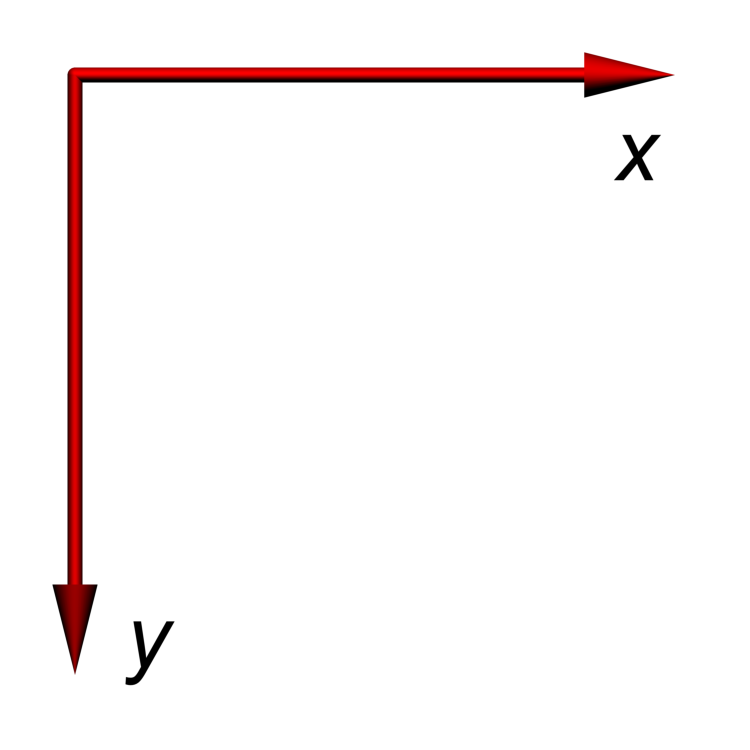
\includegraphics[scale=0.3]{coordinateSystem}
  \caption{Coordinate systems in Winforms have the $y$ axis pointing down.}
  \label{fig:coordinateSystem}
\end{figure}
%
The Screen coordinate system has its origin in the top-left corner of the screen, while the client coordinate system has its origin in the top-left corner of the drawable area of a form or a control, i.e., for a window, this will be the area without the window borders, scroll, and title bars. A control is a graphical object, such as a clickable button, will be discussed later. Conversion between client and screen coordinates is done with \idx[PointToClient@\lstinline{PointToClient}]{\lstinline{System.Drawing.PointToClient}} and \idx[PointToScreen@\lstinline{PointToScreen}]{\lstinline{System.Drawing.PointToScreen}}. %To draw geometric primitives, we must also specify the pen used for a line like primitives and the brush for filled regions.

Displaying graphics in WinForms is performed as the reaction to an event. E.g., windows are created by the program, moved, minimized, occluded by other windows, resized, etc., by the user or the program, and each action may require that the content of the window is refreshed. Thus, we must create a function that WinForms can call any time. This is known as a \idx{call-back function}, and it is added to an existing form using the form's \idx[Paint.Add@\lstinline{Paint.Add}]{\lstinline{Paint.Add}} method. Due to the event-driven nature of WinForms, functions for drawing graphics primitives are only available when responding to an event, e.g., \idx[Graphics.DrawLines@\lstinline{Graphics.DrawLines}]{\lstinline{System.Drawing.Graphics.DrawLines}} draws a line in a window, and \emph{it is only possible to call this function as part of an event handling.}

As an example, consider the problem of drawing a triangle in a window. For this we need to make a function that can draw a triangle not once, but at any amount of times as deemed necessary by the operating system. An example of such a program is shown in \Cref{winforms/triangle}.
%
\fsCode{winforms/triangle}{winforms/triangle}{Adding line graphics to a window. See \Cref{fig:triangle}}{}
%
\begin{figure}
  \centering
  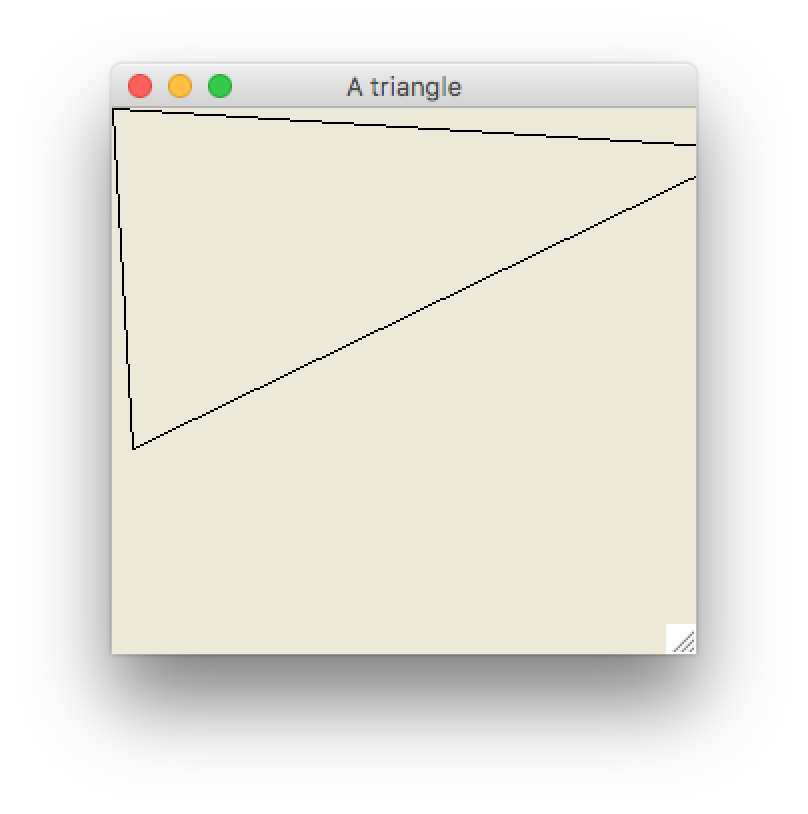
\includegraphics[scale=0.3]{triangle}
  \caption{Drawing a triangle using \Cref{winforms/triangle}.}
  \label{fig:triangle}
\end{figure}
%
A walk-through of the code is as follows: First, we open the two libraries that we will use heavily. This will save us some typing, but also pollute our namespace. E.g., now \lstinline{Point} and \lstinline{Color} are existing types, and we cannot define our own identifiers with these names. Then we create the form with size $320\times 170$, we add a paint call-back function, and we start the event-loop. The event-loop will call the paint function, whenever the system determines that the window's content needs to be refreshed. This function is to be called as a response to a paint event and takes a \lstinline!System.Windows.Forms.PaintEventArgs! object, which includes the System.Drawing.Graphics object. The function \lstinline{paint} chooses a pen and a set of points and draws a set of lines connecting the points.

The code in \Cref{winforms/triangle} is not optimal. Despite the fact that the triangle spans the rectangle $(0,0)$ to $(320,170)$ and the window's size is set to $(320,170)$, our window is too small and the triangle is clipped at the window border. The error is that we set the window's \lstinline{Size} property, which determines the size of the window including top bar and borders. Alternatively, we may set the \lstinline{ClientSize}, which determines the size of the drawable area, and this is demonstrated in \Cref{winforms/triangleClientSize} and \Cref{fig:triangleClientSize}.
%
\fsCode{winforms/triangleClientSize}{winforms/triangleClientSize}{Adding line graphics to a window. See \Cref{fig:triangleClientSize}.}{}
%
\begin{figure}
  \centering
  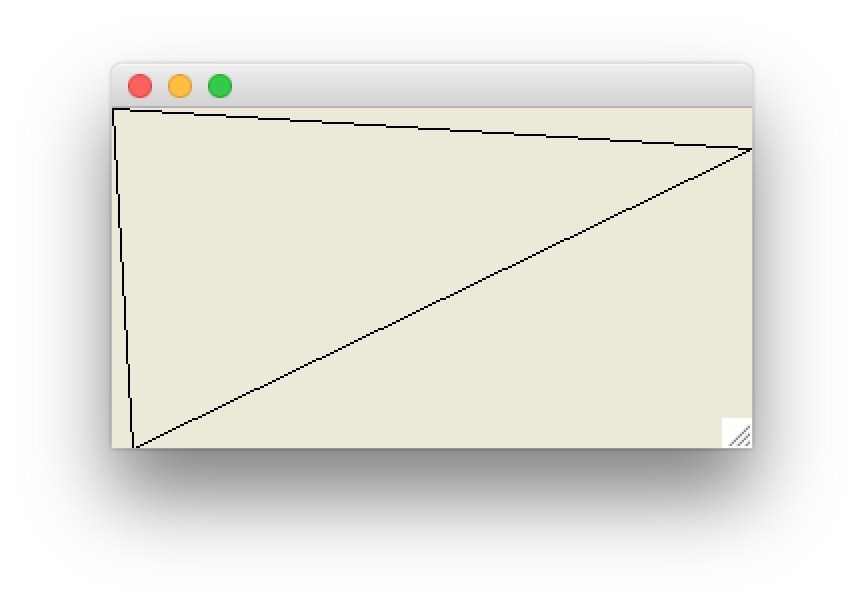
\includegraphics[scale=0.3]{triangleClientSize}
  \caption{Setting the ClientSize property gives a predictable drawing area, see \Cref{winforms/triangleClientSize} for code.}
  \label{fig:triangleClientSize}
\end{figure}
%
Thus, \advice{prefer the \lstinline{ClientSize} over the \lstinline{Size} property for internal consistency.}

Considering the program in \Cref{winforms/triangle}, we may identify a part that concerns the specification of the triangle, or more generally the graphical model, and some which concern system specific details. For future maintenance, it is often a good idea to \advice{separate the model from how it is viewed on a specific system}. E.g., it may be that at some point you decide that you would rather use a different library than WinForms. In this case, the general graphical model will be the same, but the specific details on initialization and event handling will be different. We think of the model and the viewing part of the code as top and bottom layers, respectively, and these are often connected with a connection layer. This \idx{Model-View paradigm} is shown in \Cref{fig:modelView}.
\begin{figure}
  \centering
  \begin{tikzpicture}[node distance=5mm,
    terminal/.style={
      % The shape:
      rectangle,minimum size=6mm,minimum width=30mm,rounded corners=3mm,
      % The rest
      very thick,draw=black!50,
      top color=white,bottom color=black!20,
      font=\ttfamily}]
    \node (model)  [terminal] {Model};
    \node (connection) [terminal,below=of model] {Connection};
    \node (winform) [terminal,below=of connection] {View};
    \draw[-stealth,very thick,bend left]  (model) edge (connection);
    \draw[-stealth,very thick,bend left]  (connection) edge (model);
    \draw[-stealth,very thick,bend left]  (winform) edge (connection);
    \draw[-stealth,very thick,bend left]  (connection) edge (winform);
  \end{tikzpicture}
  \caption{Separating model from view gives flexibility later.}
  \label{fig:modelView}
\end{figure}
While it is not easy to completely separate the general from the specific, it is often a good idea to strive for some degree of separation.

In \Cref{winforms/triangleOrganized}, the program has been redesigned to follow the Model-View paradigm, where \lstinline{view} contains most of the WinForms-specific code, and \lstinline{model} contains most of the geometry, which could be reused with other graphical user interfaces. The model still uses the geometric primitives from WinForms for brevity, since a general implementation of geometric primitives avoiding WinForms would have a very similar interface.
%
\fsCode{winforms/triangleOrganized}{winforms/triangleOrganized}{Improved organization of code for drawing a triangle. See \Cref{fig:triangleOrganized}.}{}
%
\begin{figure}
  \centering
  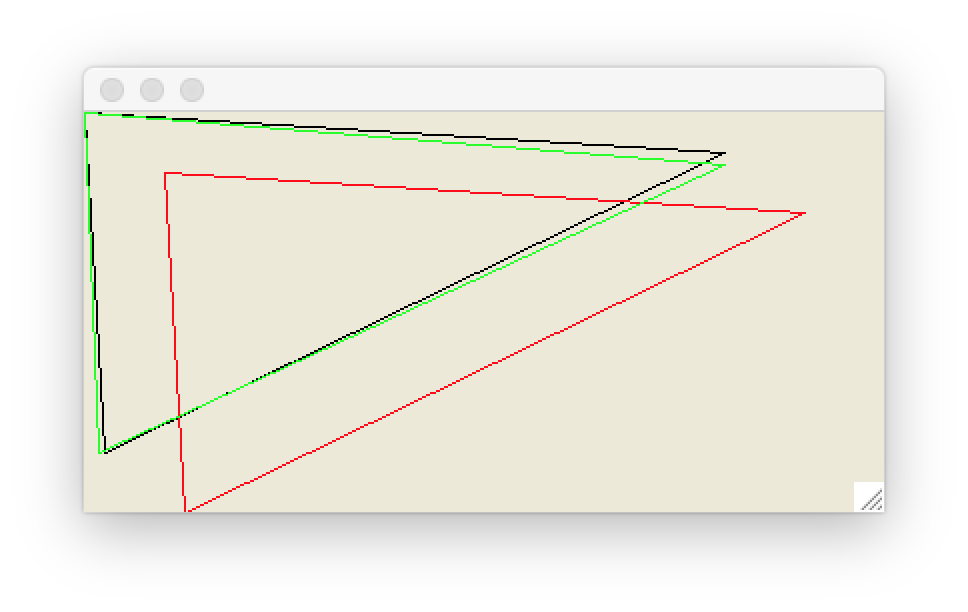
\includegraphics[scale=0.3]{triangleOrganized}
  \caption{Better organization of the code for drawing a triangle, see \Cref{winforms/triangleOrganized}.}
  \label{fig:triangleOrganized}
\end{figure}
This program is longer, but there is a much better separation of {\em what} is to be displayed (model) from {\em how} it is to be done (view).

To further our development of a general program for displaying graphics, consider the case where we are to draw another two triangles, that are a translation and rotations of the original, and where we would like to specify the color of each triangle individually. A simple extension of \lstinline{model} in \Cref{winforms/triangleOrganized} for generating many shapes of different colors is \lstinline{model : unit -> Size * ((Point []) * Pen) list}, i.e., semantically augment each point array with a pen and return a list of such pairs. For this example, we also program translation and rotation transformations. See \Cref{winforms/transformWindowsModel} for the result.
%
\fsCode{winforms/transformWindows}{winforms/transformWindowsModel}{Model of a triangle and simple transformations of it. See also \Cref{winforms/transformWindowsView,winforms/transformWindowsConnect}.}{firstline=15,firstnumber=15,lastline=43}
%
We update \lstinline{view} accordingly to iterate through this list as shown in \Cref{winforms/transformWindowsView}.
%
\fsCode{winforms/transformWindows}{winforms/transformWindowsView}{A view for lists of pairs of pen and point arrays. See also \Cref{winforms/transformWindowsModel,winforms/transformWindowsConnect}.}{lastline=13}
%
Since we are using WinForms primitives in the model, the connection layer is trivial, as shown in \Cref{winforms/transformWindowsConnect}.
%
\fsCode{winforms/transformWindows}{winforms/transformWindowsConnect}{Model of a triangle and simple transformations of it. See also \Cref{winforms/transformWindowsModel,winforms/transformWindowsView}.}{firstline=45,firstnumber=45}
% %
% \begin{figure}
%   \centering
%   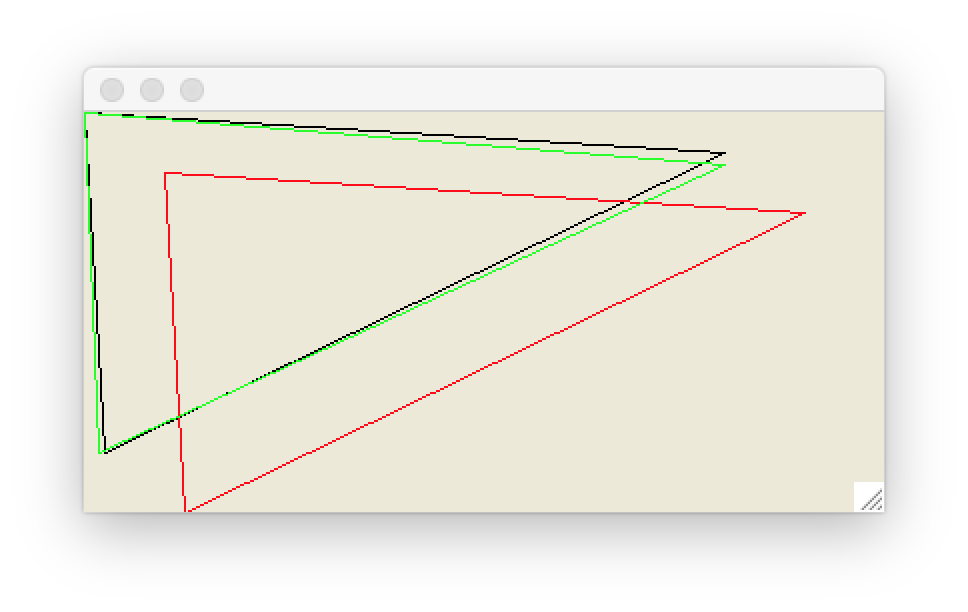
\includegraphics[scale=0.3]{transformWindows}
%   \caption{Transformed versions of the same triangle resulting from running the code in \Crefrange{winforms/transformWindowsModel}{winforms/transformWindowsConnect}.}
%   \label{fig:transformWindow}
% \end{figure}

% We now have a basis for solving the following problem:
% \begin{task}
%   Given a triangle produce a Mandela drawing, where $n$ rotated versions of the triangle is drawn around its center of mass.
% \end{task}
% Reusing the top part of \filename{transformWindows.fsx} (\Cref{winforms/transformWindowsModel}) and replacing the bottom part with the code shown in \Cref{winforms/rotationalSymmetry}, we arrive a the solution illustrated in \Cref{fig:rotationalSymmetry}.
% %
% \fsCode{winforms/rotationalSymmetry}{winforms/rotationalSymmetry}{Create the window and changing its properties. Last part is ommitted, since it is identical to \Cref{winforms/transformWindowsBottom}.}{lastline=51}
% %
% \begin{figure}
%   \centering
%   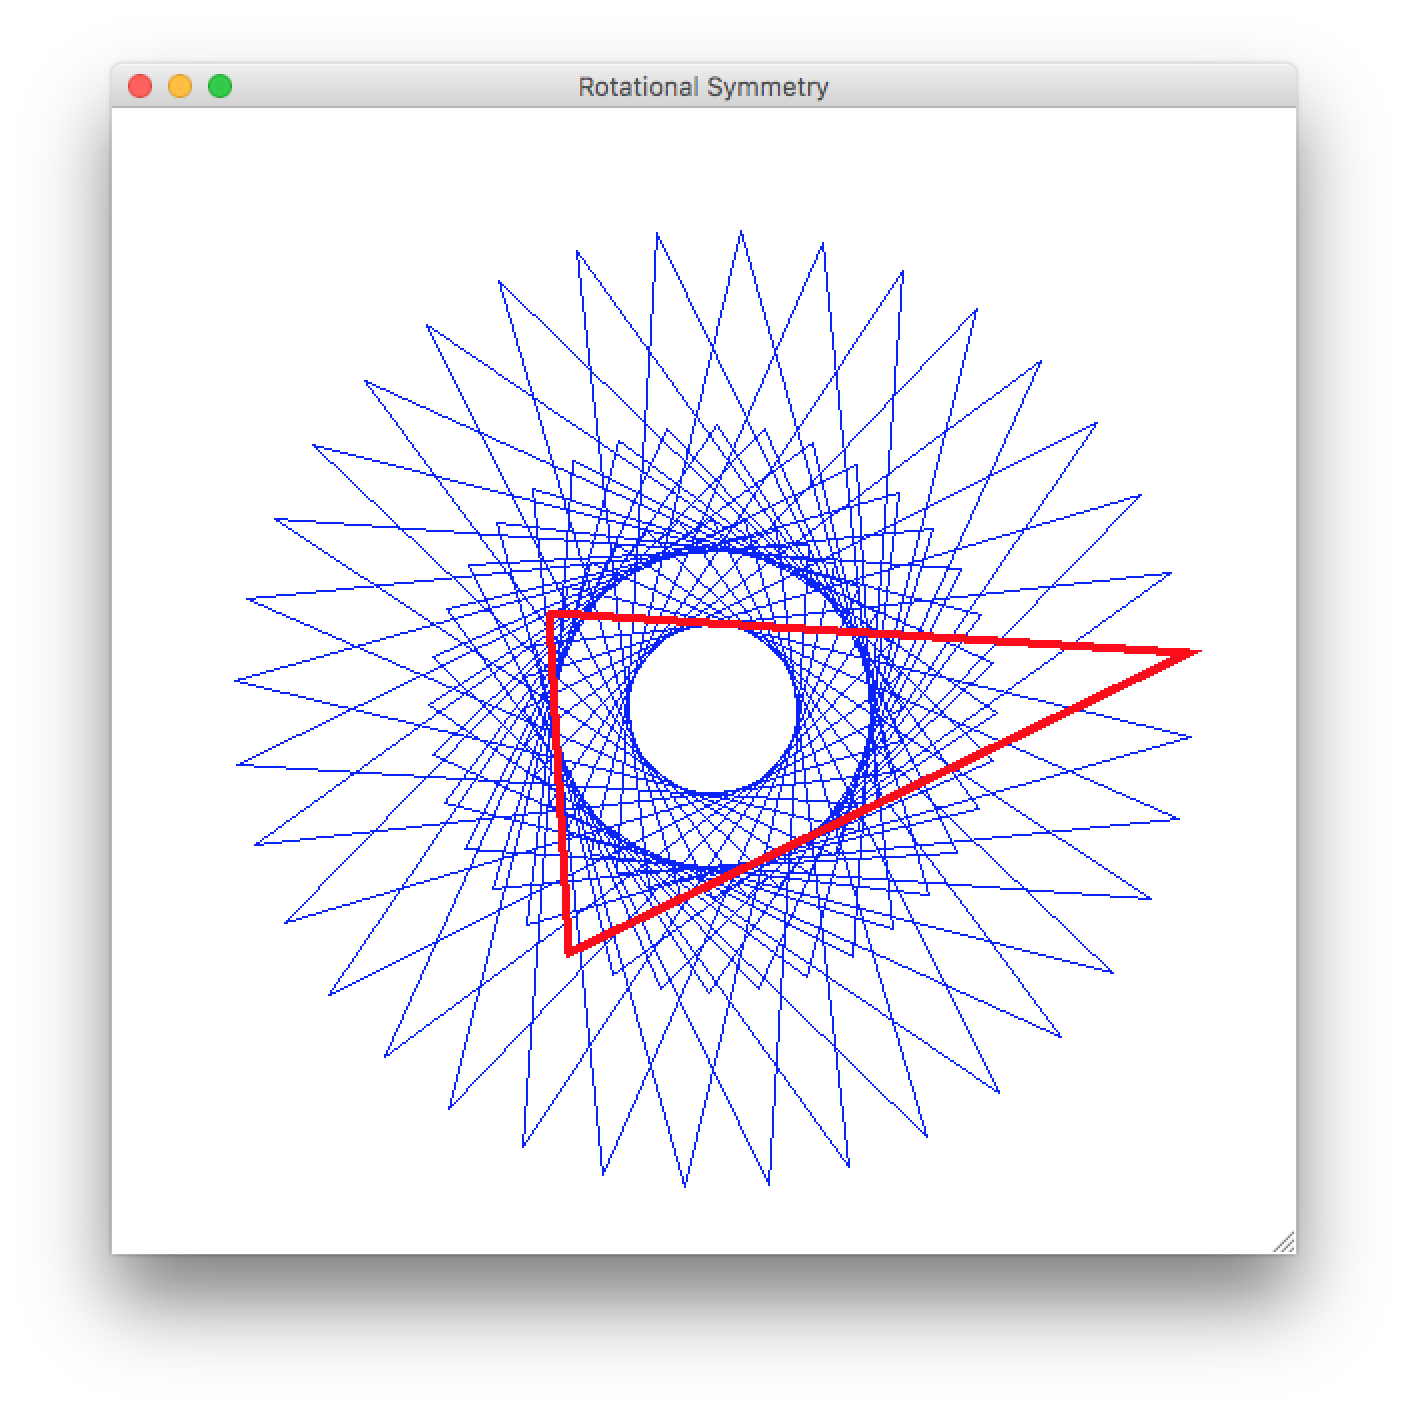
\includegraphics[width=0.8\textwidth]{rotationalSymmetry}
%   \caption{A symmetric figure resulting from \Cref{winforms/rotationalSymmetry}.}
%   \label{fig:rotationalSymmetry}
% \end{figure}

% The \lstinline!System.Drawing.Graphics! class contains many other algorithms for drawing graphics primitives, some of which are listing in \Cref{tab:graphicsMethods}
% \begin{table}
%   \begin{center}
%   \rowcolors{2}{oddRowColor}{evenRowColor}
%     \begin{tabularx}{\linewidth}{|l|X|}
%       \hline
%       \rowcolor{headerRowColor}  Function & Description\\
%       \hline
%       \lstinline{DrawArc : Pen * Rectangle * Single * Single}
%       &Draws an arc representing a portion of an ellipse specified by a Rectangle structure.\\
%       \hline
%       \lstinline{DrawBezier : Pen * Point * Point * Point * Point}    
%       &Draws a Bézier spline defined by four Point structures.\\
%       \hline
%       \lstinline{DrawCurve : Pen * Point[]}    
%       &Draws a cardinal spline through a specified array of Point structures.\\
%       \hline
%       \lstinline{DrawEllipse : Pen * Rectangle}    
%       &Draws an ellipse specified by a bounding Rectangle structure.\\
%       \hline
%       \lstinline{DrawImage : Image * Point[]}    
%       &Draws the specified Image at the specified location and with the specified shape and size.\\
%       \hline
%       \lstinline{DrawLine : Pen * Point * Point}    
%       &Draws a series of line segments that connect an array of Point structures.\\
%       \hline
%       \lstinline{DrawLines : Pen * Point[]}    
%       &Draws a series of line segments that connect an array of Point structures.\\
%       \hline
%       \lstinline{DrawPie : Pen * Rectangle * Single * Single}    
%       &Draws a pie shape defined by an ellipse specified by a Rectangle structure and two radial lines.\\
%       \hline
%       \lstinline{DrawPolygon : Pen * Point[]}    
%       &Draws a polygon defined by an array of Point structures.\\
%       \hline
%       \lstinline{DrawRectangles : Pen * Rectangle[]}    
%       &Draws a series of rectangles specified by Rectangle structures.\\
%       \hline
%       \lstinline{DrawString : string * Font * Brush * PointF}    
%       &Draws the specified text string at the specified location with the specified Brush and Font objects.\\
%       \hline
%       \lstinline{FillClosedCurve : Brush * Point[]}    
%       &Fills the interior of a closed cardinal spline curve defined by an array of Point structures.\\
%       \hline
%       \lstinline{FillEllipse : Brush * Rectangle}    
%       &Fills the interior of an ellipse defined by a bounding rectangle specified by a Rectangle structure.\\
%       \hline
%       \lstinline{FillPie : Brush * Rectangle * Single * Single}    
%       &Fills the interior of a pie section defined by an ellipse specified by a RectangleF structure and two radial lines.\\
%       \hline
%       \lstinline{FillPolygon : Brush * Point[]}    
%       &Fills the interior of a polygon defined by an array of points specified by Point structures.\\
%       \hline
%       \lstinline{FillRectangle : Brush * Rectangle}    
%       &Fills the interior of a rectangle specified by a Rectangle structure.\\
%       \hline
%     \end{tabularx}
%   \end{center}
%   \caption{Some methods of the \lstinline!System.Drawing.Graphics! class.}
%   \label{tab:graphicsMethods}
% \end{table}
% \jon{Give examples of more methods}
\clearpage % The figures are having trouble interacting with listings

\section{Programming Intermezzo: Hilbert Curve}
A curve in 2 dimensions has a length but no width, and we can only visualize it by giving it a width. Thus, it came as a surprise to many when Giuseppe Peano in 1890 demonstrated that there exist curves which fill every point in a square. The method he used to achieve this was recursion:
\begin{task}
  Consider a curve consisting of piecewise straight lines all with the same length but with varying angles $0^{\circ}$, $90^{\circ}$, $180^{\circ}$, or $270^{\circ}$ w.r.t.\ the horizontal axis. To draw this curve, we need 3 basic operations: Move forward ($F$), turn right (R), and turn left (L). The turning is w.r.t.\ the present direction. A Hilbert Curve is a space-filling curve which can be expressed recursively as:
\begin{align}
  A &\rightarrow LBFRAFARFBL,\label{eq:hilbertA}\\
  B &\rightarrow RAFLBFBLFAR,\label{eq:hilbertB}
\end{align}
starting with $A$. For practical illustrations, we typically only draw space-filling curves to a specified depth of recursion, which is called the order of the curve. To keep track of the level of recursion, we introduce an index as:
\begin{align*}
  A_{n+1} &\rightarrow LB_nFRA_nFA_nRFB_nL,\\
  B_{n+1} &\rightarrow RA_nFLB_nFB_nLFA_nR,
\end{align*}
for $n>0$ and $A_0\rightarrow\emptyset$ and $B_0\rightarrow\emptyset$. Thus, the first-order curve is
\begin{align*}
  A_1 \rightarrow LB_0FRA_0FA_0RFB_0L \rightarrow LFRFRFL,
\end{align*}
and the second order curve is
\begin{align*}
  A_2 
  \rightarrow &LB_1FRA_1FA_1RFB_1L \\
  \rightarrow &LRFLFLFRFRLFRFRFLFLFRFRFLRFRFLFLFRL.
\end{align*}
Since $LR = RL = \emptyset$ the above simplifies to
\begin{align*}
  A_2 \rightarrow FLFLFRFFRFRFLFLFRFRFFRFLFLF
\end{align*}
Make a program that given an order produces an image of the Hilbert curve.
\end{task}
Our strategy to solve this problem will be first to define the curves in terms of movement commands $LRFL\ldots$. For this, we will define a discriminated union
\lstinline{type Command = F | L | R}. The movement commands can then be defined as a \lstinline{Command list} type. The list for a specific order is a simple set of recursive functions in F\# which we will call \lstinline{A} and \lstinline{B}.

To produce a graphical drawing of a command list, we must transform it into coordinates, and during the conversion, we need to keep track of both the present position and the present heading, since not all commands draw. This is a concept similar to Turtle Graphics, which is often associated with the Logo programming language from the 1960's. In Turtle graphics, we command a little robot - a turtle - which moves in 2 dimensions and can turn on the spot or move forward, and its track is the line being drawn. Thus we introduce a \lstinline!type Turtle = {x : float; y : float; d : float}! record. Conversion of command lists to turtle lists is a fold programming structure, where the command list is read from left-to-right, building up an accumulator by adding each new element. For efficiency, we choose to prepend the new element to the accumulator. This we have implemented as the \lstinline{addRev} function. Once the full list of turtles has been produced, then it is reversed.

Finally, the turtle list is converted to WinForms \lstinline{Point} array, and a window of appropriate size is chosen. The resulting model part is shown in \Cref{hilbertModel}. The view and connection parts are identical to \Cref{winforms/transformWindowsView,winforms/transformWindowsConnect}, and \Cref{fig:hilbert} shows the result of using the program to draw Hilbert curves of orders 1, 2, 3, and 5.
%
\fsCode{winforms/hilbert}{hilbertModel}{Using simple turtle graphics to produce a list of points on a polygon. The code continues in Listing~\ref{hilbertModelCont}. The view and connection parts are identical to \Cref{winforms/transformWindowsView,winforms/transformWindowsConnect}.}{firstline=15,firstnumber=15,lastline=46}
%
\fsCode{winforms/hilbert}{hilbertModelCont}{Continued from Listing~\ref{hilbertModel}.}{firstline=48,firstnumber=48,lastline=63}
%
\begin{figure}
  \centering
  \subfigure[Order 1]{
\includegraphics[scale=0.3]{hilbert1}}
  \subfigure[Order 2]{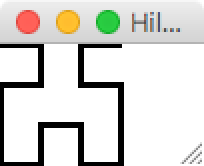
\includegraphics[scale=0.3]{hilbert2}}
  \subfigure[Order 3]{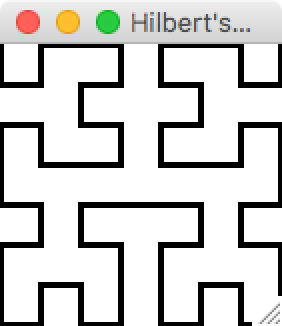
\includegraphics[scale=0.3]{hilbert3}}
  \subfigure[Order 5]{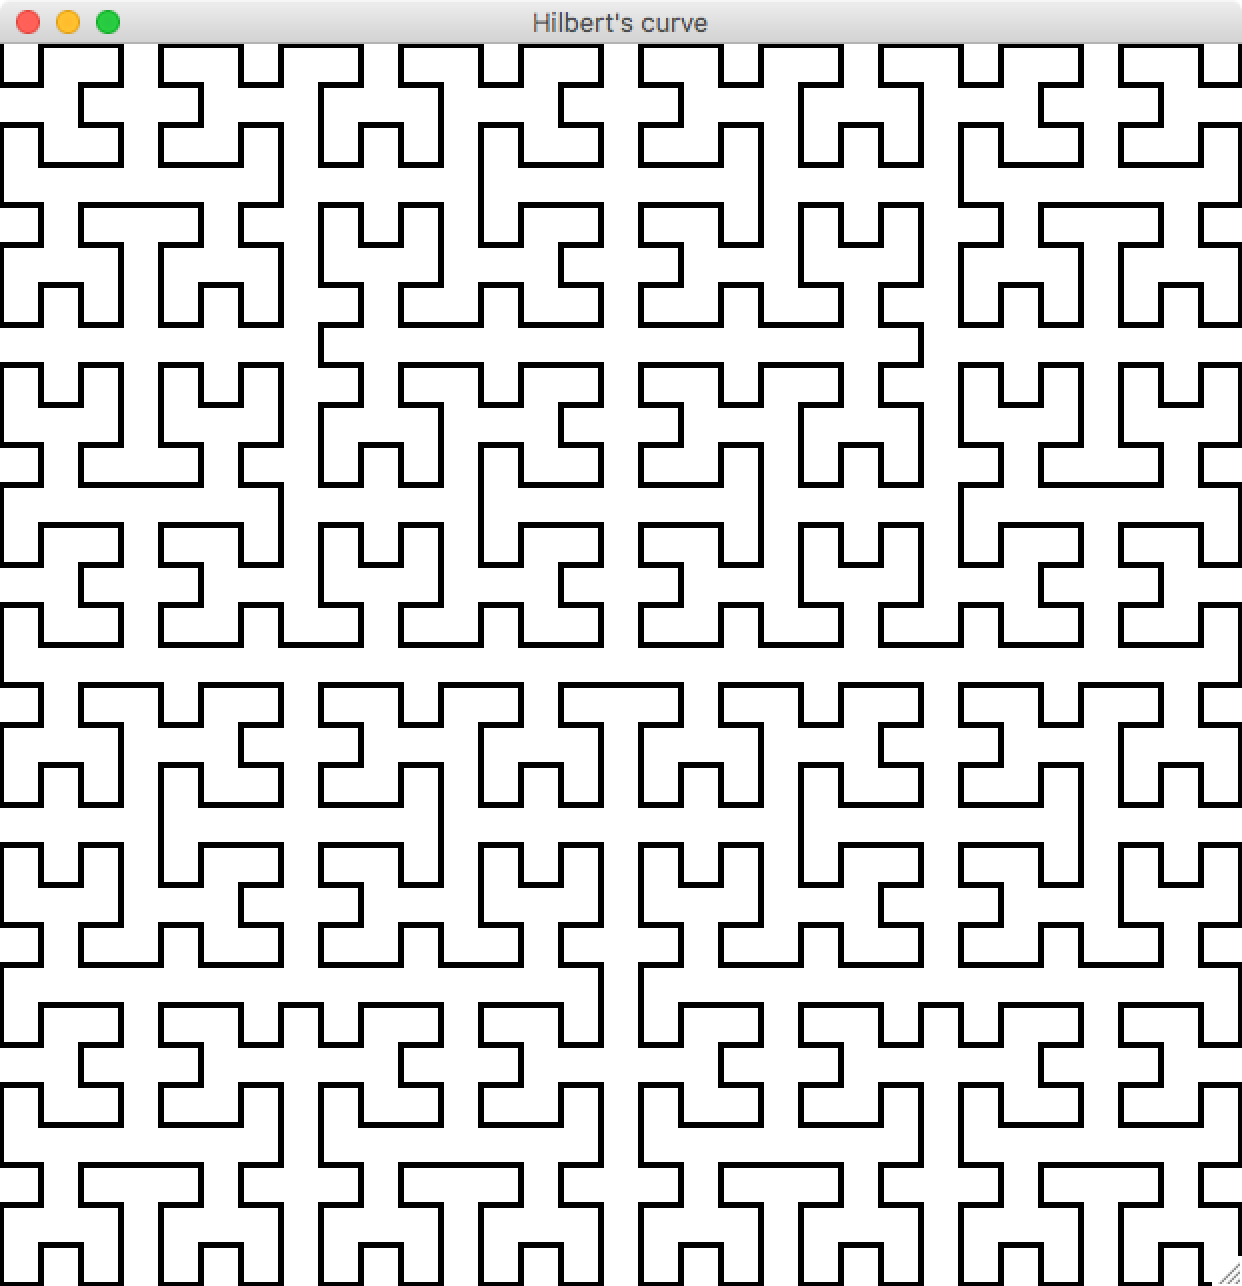
\includegraphics[scale=0.3]{hilbert5}}
  \caption{Hilbert curves of orders 1, 2, 3, and 5 by code in \Cref{hilbertModel}.}
  \label{fig:hilbert}
\end{figure}
\clearpage % The figures are having trouble interacting with listings

\section{Handling Events}
In the previous section, we have looked at how to draw graphics using the \lstinline!Paint! method of an existing form object. Forms have many other event handlers that we may use to interact with the user. \Cref{winforms/windowEventsCode} demonstrates event handlers for moving and resizing a window, for clicking in a window, and for typing on the keyboard. 
%
\fsCode{winforms/windowEvents}{winforms/windowEventsCode}{Catching window, mouse, and keyboard events.}{}
%
\fsOutput{winforms/windowEvents}{Output from an interaction with the program in \Cref{winforms/windowEventsCode}.}
%
\Cref{winforms/windowEventsCode} shows the output from an interaction with the program which is the result of the following actions: moving the window, resizing the window, clicking the left mouse key, pressing and holding the down the left mouse key while moving the mouse, releasing the left mouse key, and typing ``abc''. As demonstrated, some actions, like moving the mouse, result in a lot of events, and some, like the initial window moves results, are surprising. Thus, event-driven programming should take care to interpret the events robustly and carefully.

Common for all event-handlers is that they listen for an event, and when the event occurs, the functions that have been added using the \lstinline{Add} method are called. This is also known as sending a message. Thus, a single event can give rise to calling zero or more functions.

Graphical user interfaces and other systems often need to perform actions that depend on specific lengths of time or a certain point in time. To measure length of time F\# has the \idx[Timer@\lstinline{Timer}]{\lstinline{System.Windows.Forms.Timer}} class, which technically is an optimized of \lstinline{System.Timers.Timer} for graphical user interfaces. The Timer class can be used to create an event after a specified duration of time. F\# also has the \idx[DateTime@\lstinline{DateTime}]{\lstinline{System.DateTime}} class to specify points in time. An often used property is \lstinline{System.DateTime.Now}, which returns a \lstinline{DateTime} object for the date and time when the property is accessed. The use of these two classes is demonstrated in \Cref{winforms/clock} and \Cref{fig:clock}.
%
\fsCode{winforms/clock}{winforms/clock}{Using \lstinline{System.Windows.Forms.Timer} and \lstinline{System.DateTime.Now} to update the display of the present date and time. See \Cref{fig:clock} for the result.}{}
%
\begin{figure}
  \centering
  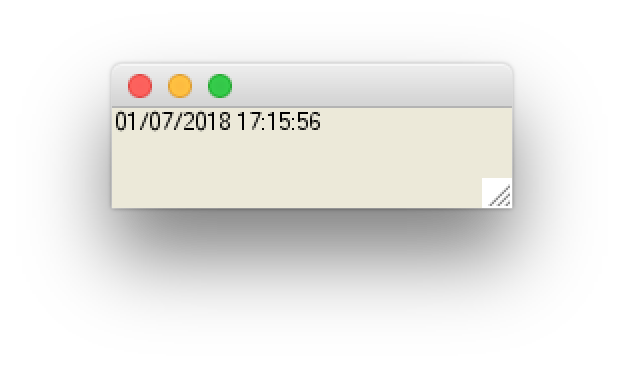
\includegraphics[scale=0.3]{clock}
  \caption{See \Cref{winforms/clock}.}
  \label{fig:clock}
\end{figure}
In the code, a label has been created to show the present date and time. The label is a type of control, and it is displayed using the default font which is rather small. How to change this and other details on controls will be discussed in the next section.

In the example, the label is redrawn everytime the text is changed, such that the current value is correctly displayed on the screen. Sometimes it is necessary to force a control to redraw which can be done with the \lstinline{Refresh()} method. Since a \lstinline{Form} is also a type of control, it is common to trigger a redraw event for the top form, which in \Cref{winforms/clock} would be \lstinline{win.Refresh()}. Thus, \lstinline{Refresh()} and a \lstinline{Timer} object can be used to produce animations.

% %
% \fsCode{winforms/refresh}{winforms/refresh}{\dots}{}
% %
% \begin{figure}
%   \centering
%   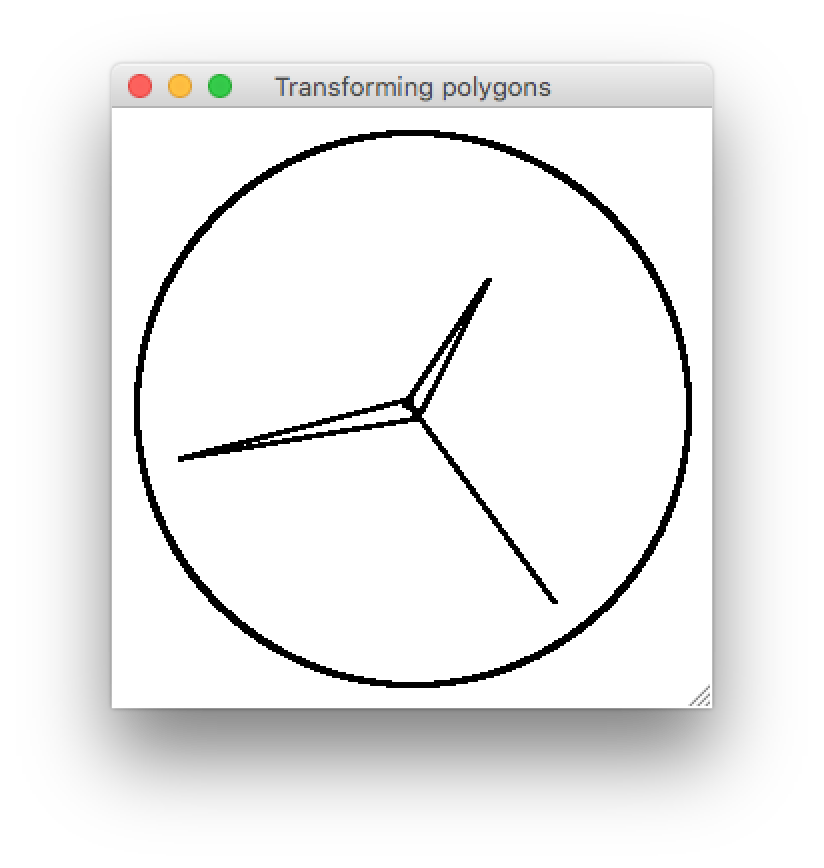
\includegraphics[width=0.3\textwidth]{analogueClock}
%   \caption{See \Cref{winforms/refresh}.}
%   \label{fig:refresh}
% \end{figure}
\clearpage

\section{Labels, Buttons, and Pop-up Windows}
In WinForms, buttons, menus and other interactive elements are called \idx[control]{Controls}. A form is a type of control, and thus, programming controls are very similar to programming windows. \Cref{winforms/buttonControl} shows a small program that displays a label and a button in a window, and when the button is pressed, then the label is updated.
%a dialogue is opened in another window. \Cref{fig:buttonControl} shows an example dialogue.
%
\fsCode{winforms/buttonControl}{winforms/buttonControl}{Create the button and an event, see also \Cref{fig:buttonControl}.}{}
%
\begin{figure}
  \centering
  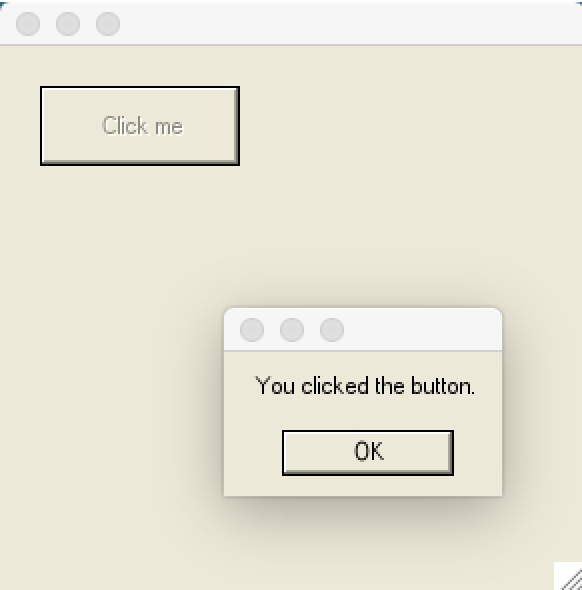
\includegraphics[scale=0.3]{buttonControl}
  \caption{After pressing the button 3 times. See \Cref{winforms/buttonControl}.}
  \label{fig:buttonControl}
\end{figure}
%
As the listing demonstrates, the button is created using the \idx[Button@\lstinline{Button}]{\lstinline{System.Windows.Forms.Button}} constructor, and it is added to the window's form's control list. The \lstinline{Location} property controls its position w.r.t.\ the enclosing form. Other accessors are \lstinline{Width}, \lstinline{Text}, and \lstinline{Size}.

\lstinline{System.Windows.Forms} includes a long list of controls, some of which are summarized in \Cref{tab:controls}.\idxs{CheckBox@\lstinline{CheckBox}}\idxs{DateTimePicker@\lstinline{DateTimePicker}}\idxs{Label@\lstinline{Label}}\idxs{ProgressBar@\lstinline{ProgressBar}}\idxs{RadioButton@\lstinline{RadioButton}}\idxs{TextBox@\lstinline{TextBox}}
\begin{table}
  \begin{center}
  \rowcolors{2}{oddRowColor}{evenRowColor}
    \begin{tabularx}{\linewidth}{|l|X|}
      \hline
      \rowcolor{headerRowColor}  Method/Property & Description\\
      \hline
      \lstinline{Button}
      &A clickable button.\\
      \hline
      \lstinline{CheckBox}
      &A clickable check box.\\
      \hline
      \lstinline{DateTimePicker}
      &A box showing a date with a drop-down menu for choosing another.\\
      \hline
      \lstinline{Label}
      &A displayable text.\\
      \hline
      \lstinline{ProgressBar}
      &A box showing a progress bar.\\
      \hline
      \lstinline{RadioButton}
      &A single clickable radio button. Can be paired with other radio buttons.\\
      \hline
      \lstinline{TextBox}
      &A text area, which can accept input from the user.\\
      \hline
    \end{tabularx}
  \end{center}
  \caption{Some types of \lstinline{System.Windows.Forms.Control}.}
  \label{tab:controls}
\end{table}
Examples are given in \lstinline{controls}, shown in \Cref{winforms/controls} and \Cref{fig:controls}.
%
\fsCode{winforms/controls}{winforms/controls}{Examples of control elements added to a window form, see also \Cref{fig:controls}.}{}
%
\begin{figure}
  \centering
  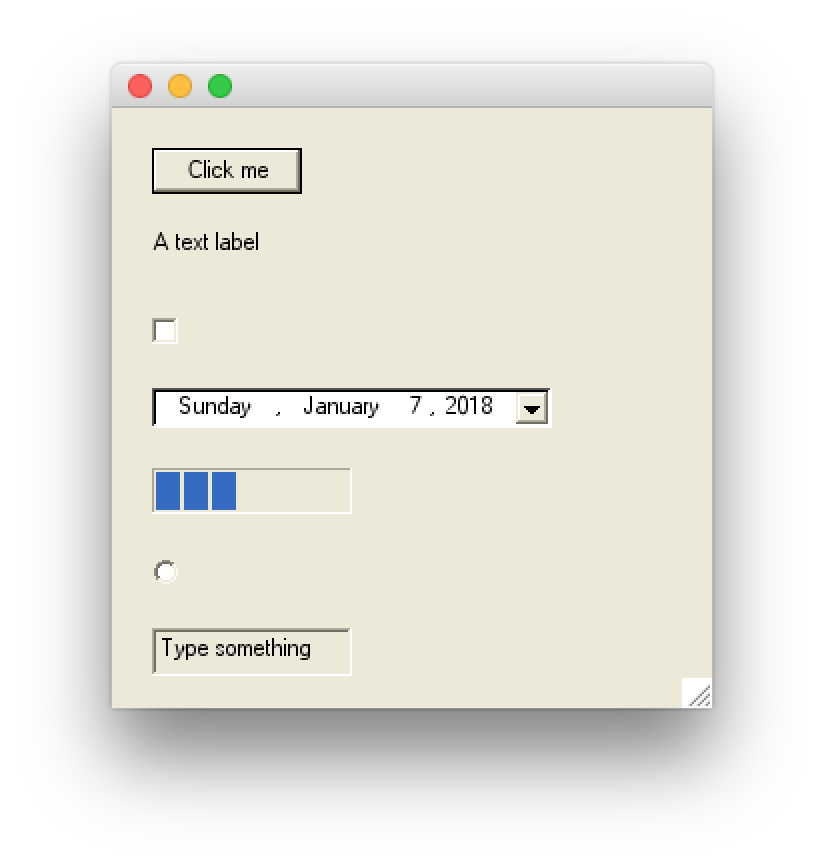
\includegraphics[scale=0.3]{controls}
  \caption{Examples of control elements. See \Cref{winforms/controls}.}
  \label{fig:controls}
\end{figure}

Some controls open separate windows for more involved dialogue with the user. Some examples are \lstinline{MessageBox}, \lstinline{OpenFileDialog}, and \lstinline{SaveFileDialog}.

\idx[MessageBox@\lstinline{MessageBox}]{\lstinline{System.Windows.Forms.MessageBox}} is used to have a simple but restrictive dialogue with the user, which is demonstrated in \Cref{winforms/messageBox} and \Cref{fig:MessageBox}.
%
\fsCode{winforms/messageBox}{winforms/messageBox}{Create the \lstinline{MessageBox}, see also \Cref{fig:MessageBox}.}{}
%
\begin{figure}
  \centering
  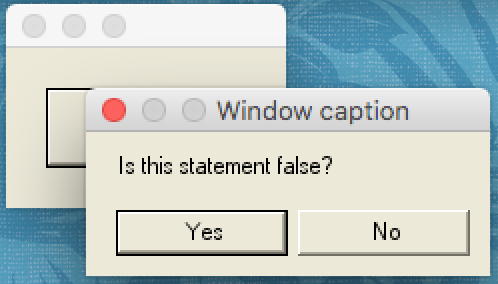
\includegraphics[scale=0.5]{MessageBox}
  \caption{After pressing the ``Click-me'' button. See \Cref{winforms/messageBox}.}
  \label{fig:MessageBox}
\end{figure}
%
As an alternative to the \lstinline{YesNo} response button, the message box also offers \lstinline{AbortRetryIgnore}, \lstinline{OK}, \lstinline{OKCancel}, \lstinline{RetryCancel}, and \lstinline{YesNoCancel}. Note that all other windows of the process are blocked until the user closes the dialogue window.

With \idx[OpenFileDialog@\lstinline{OpenFileDialog}]{\lstinline{System.Windows.Forms.OpenFileDialog}}, you can ask the user to select an existing filename, as demonstrated in \Cref{winforms/openFileDialog} and \Cref{fig:openFileDialog}.
%
\fsCode{winforms/openFileDialog}{winforms/openFileDialog}{Create the \lstinline{OpenFileDialog}, see also \Cref{fig:openFileDialog}.}{}
%
\begin{figure}
  \centering
  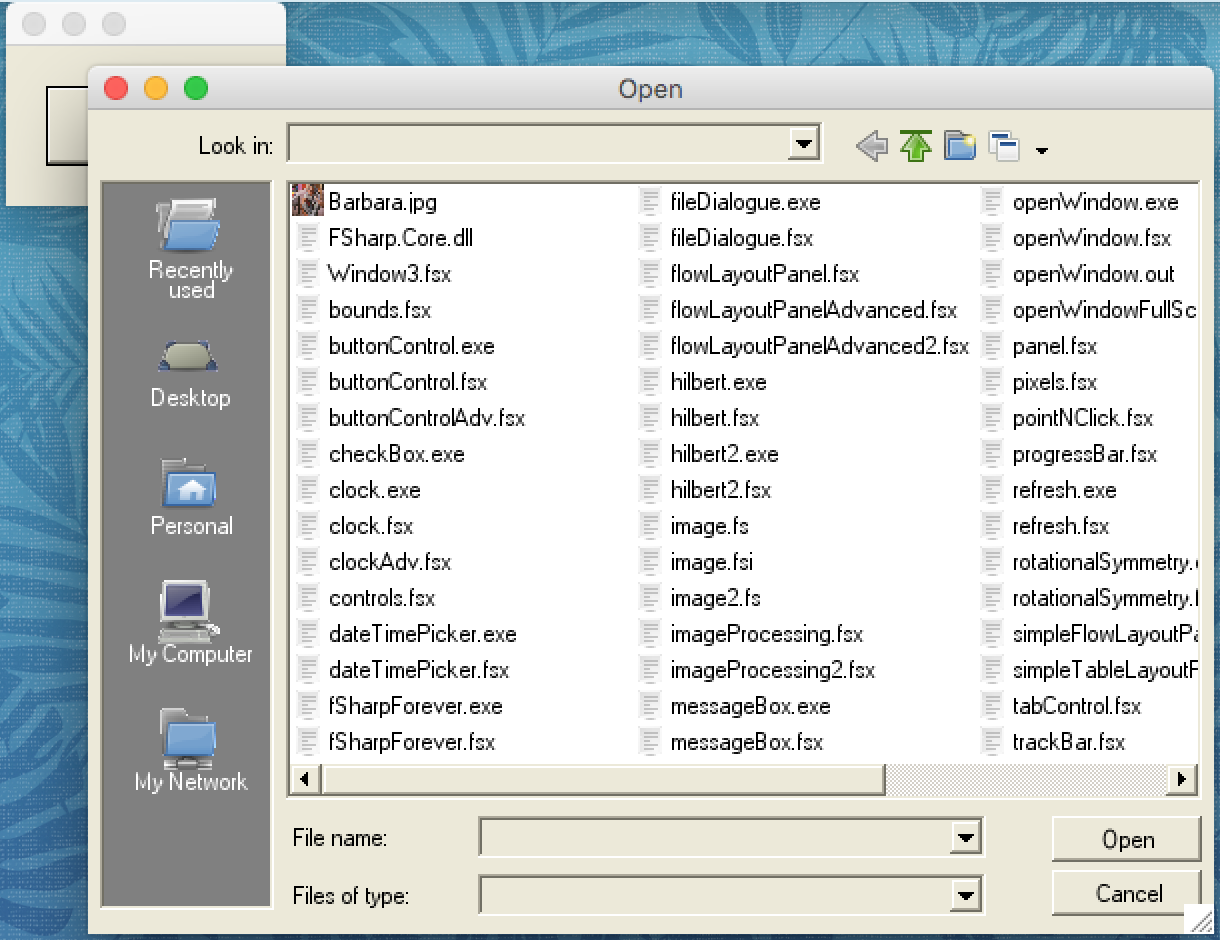
\includegraphics[scale=0.5]{openFileDialog}
  \caption{Ask the user for a filename to read from. See \Cref{winforms/openFileDialog}.}
  \label{fig:openFileDialog}
\end{figure}
%
Similarly to \lstinline{OpenFileDialog}, \idx[SaveFileDialog@\lstinline{SaveFileDialog}]{\lstinline{System.Windows.Forms.SaveFileDialog}} asks for a file name, but if an existing file is selected, then the user will be asked to confirm the choice.
\clearpage

\section{Organizing Controls}
It is often useful to organize the controls in groups, and such groups are called \idx{Panels} in WinForms. An example of creating a \lstinline{System.Windows.Forms.Panel} that includes a \lstinline{System.Windows.Forms.TextBox} and \lstinline{System.Windows.Forms.Label} for getting user input is shown in \Cref{winforms/panel} and \Cref{fig:panel}. 
%
\fsCode{winforms/panel}{winforms/panel}{Create a panel, label, and text input controls.}{}
%
\begin{figure}
  \centering
  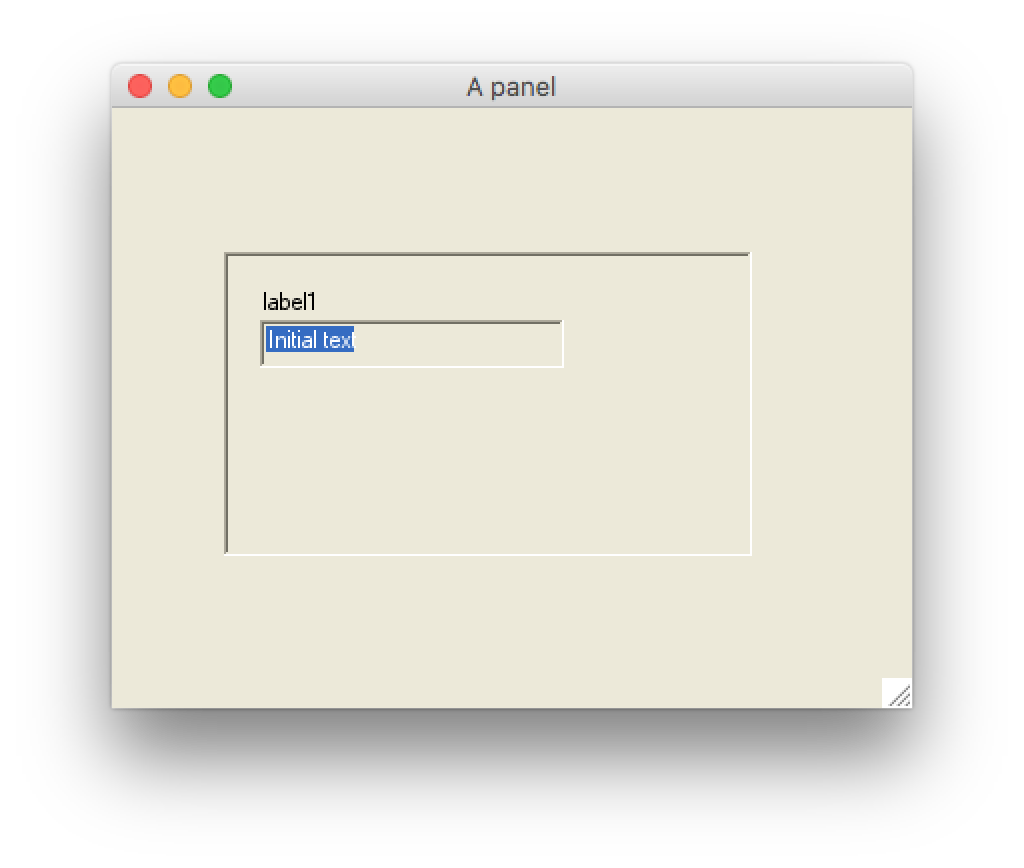
\includegraphics[scale=0.3]{panel}
  \caption{A panel including a label and a text input field, see \Cref{winforms/panel}.}
  \label{fig:panel}
\end{figure}
The label and textbox are children of the panel, and the main advantage of using panels is that the coordinates of the children are relative to the top left corner of the panel. I.e., moving the panel will move the label and the textbox at the same time.

A very flexible panel is the \idx[FlowLayoutPanel@\lstinline{FlowLayoutPanel}]{\lstinline{System.Windows.Forms.FlowLayoutPanel}}, which arranges its objects according to the space available. This is useful for graphical user interfaces targeting varying device sizes, such as a computer monitor and a tablet, and it also allows the program to gracefully adapt when the user changes window size. A demonstration of \lstinline{System.Windows.Forms.FlowLayoutPanel} together with \lstinline{System.Windows.Forms.CheckBox} and \lstinline{System.Windows.Forms.RadioButton} is given in \Crefrange{winforms/flowLayoutPanelTop}{winforms/flowLayoutPanel} and in \Cref{fig:flowLayoutPanel}. The program illustrates how the button elements flow under four possible flow directions with \lstinline{System.Windows.FlowDirection}, and how \lstinline{System.Windows.WrapContents} influences what happens to content that flows outside the panel's region. 
%
\fsCode{winforms/flowLayoutPanel}{winforms/flowLayoutPanelTop}{Create a FlowLayoutPanel with checkbox and radio buttons.}{lastline=34}
%
\fsCode{winforms/flowLayoutPanel}{winforms/flowLayoutPanel}{Create a FlowLayoutPanel with checkbox and radio buttons. Continued from \Cref{winforms/flowLayoutPanelTop}.}{firstline=36,firstnumber=36}
%
\begin{figure}
  \centering
  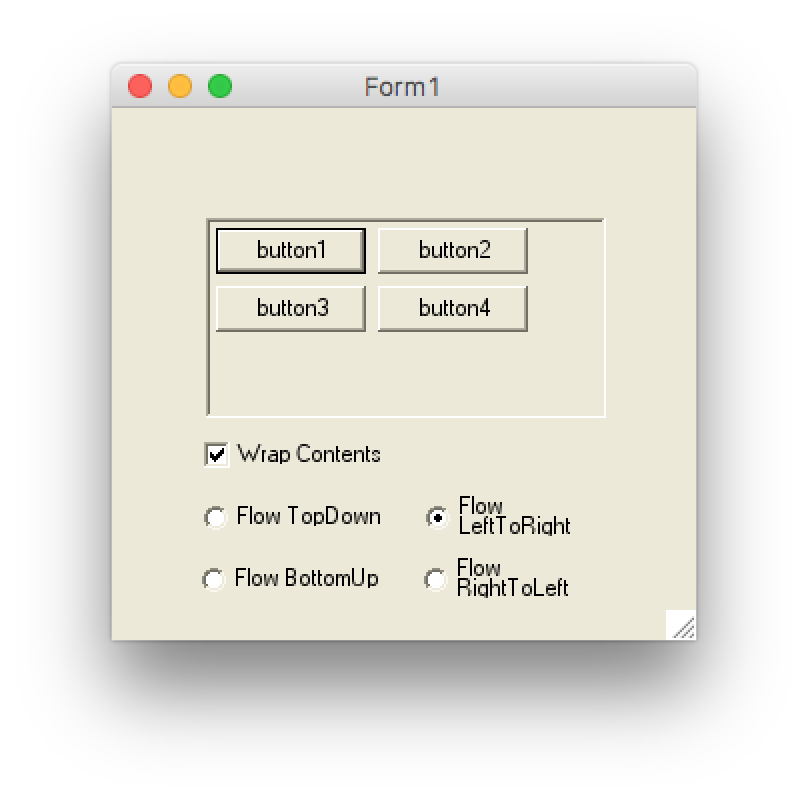
\includegraphics[scale=0.3]{flowLayoutPanel}
  \caption{Demonstration of the \lstinline!FlowLayoutPanel! panel, \lstinline!CheckBox!, and \lstinline!RadioButton! controls, see \Crefrange{winforms/flowLayoutPanelTop}{winforms/flowLayoutPanel}.}
  \label{fig:flowLayoutPanel}
\end{figure}
A walkthrough of the program is as follows. The goal is to make 2 areas, one giving the user control over display parameters, and another displaying the result of the user's choices. These are \lstinline{FlowLayoutPanel} and \lstinline{Panel}. In the \lstinline{FloatLayoutPanel} there are four \lstinline{Button}s to be displayed in a region that is not tall enough for the buttons to be shown in vertical sequence and not wide enough to be shown in horizontal sequence. Thus the \lstinline{FlowDirection} rules come into play, i.e., the buttons are added in sequence as they are named, and the default \lstinline{FlowDirection.LeftToRight} arranges the \lstinline{buttonLst[0]} in the top left corner, and \lstinline{buttonLst[1]} to its right. Other flow directions do it differently, and the reader is encouraged to experiment with the program.

The program in \Cref{winforms/flowLayoutPanel} has not completely separated the semantic blocks of the interface and relies on explicit setting of coordinates of controls. This can be avoided by using nested panels. E.g., in \Crefrange{winforms/flowLayoutPanelAdvancedTop}{winforms/flowLayoutPanelAdvanced}, the program has been rewritten as a nested set of \lstinline{FloatLayoutPanel} in three groups: The button panel, the checkbox, and the radio button panel. Adding a \lstinline{Resize} event handler for the window to resize the outermost panel according to the outer window allows for the three groups to change position relative to each other. This results in three different views, all shown in \Cref{fig:flowLayoutPanelAdvanced}.
%
\fsCode{winforms/flowLayoutPanelAdvanced}{winforms/flowLayoutPanelAdvancedTop}{Create nested FlowLayoutPanel.}{lastline=42}
%
\fsCode{winforms/flowLayoutPanelAdvanced}{winforms/flowLayoutPanelAdvanced}{Create nested FlowLayoutPanel. Continued from \Cref{winforms/flowLayoutPanelAdvancedTop}.}{firstline=44,firstnumber=44}
%
\begin{figure}
  \centering
  \subfigure[]{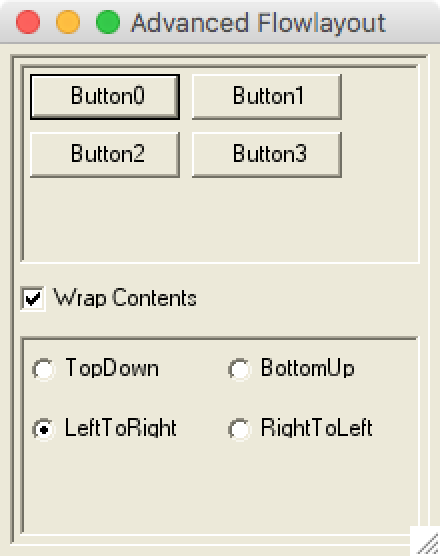
\includegraphics[scale=0.3]{flowLayoutPanelAdvanced}}
  \subfigure[]{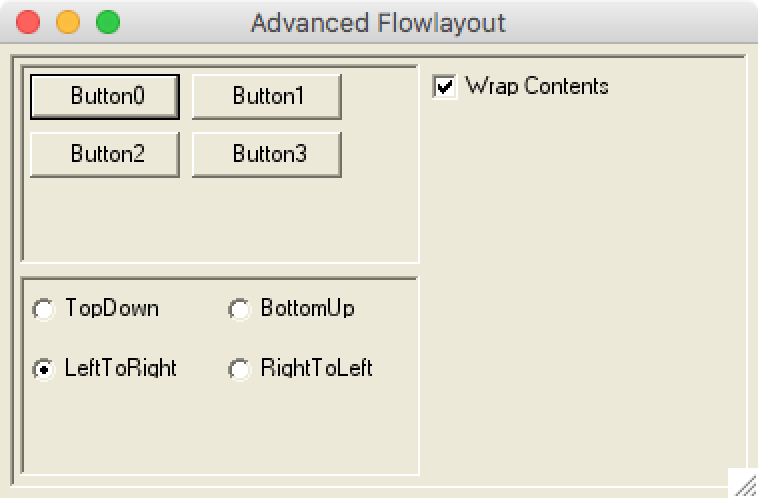
\includegraphics[scale=0.3]{flowLayoutPanelAdvanced2}}
  \subfigure[]{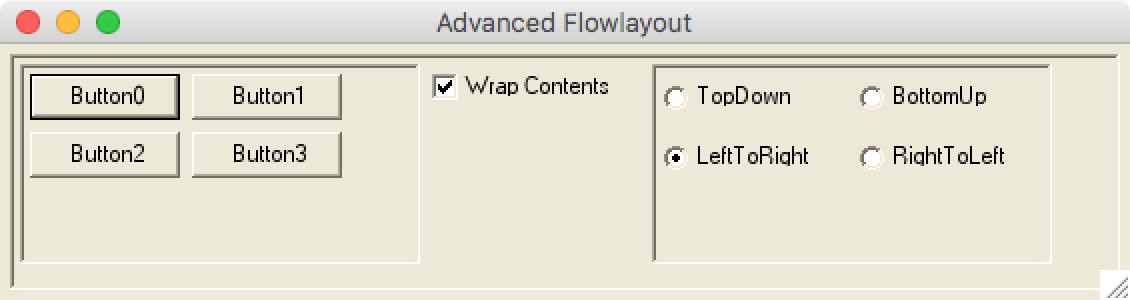
\includegraphics[scale=0.3]{flowLayoutPanelAdvanced3}}
  \caption{Nested \lstinline!FlowLayoutPanel!, see \Crefrange{winforms/flowLayoutPanelAdvancedTop}{winforms/flowLayoutPanelAdvanced}, allows for dynamic arrangement of content. Content flows when the window is resized.}
  \label{fig:flowLayoutPanelAdvanced}
\end{figure}
%\jon{Add simple panel code \lstinline!simpleFlowLayoutPanel.fsx! and \lstinline!simpleTableLayoutPanel.fsx!.}  
%\jon{Add \lstinline{Dock}, \lstinline{Padding} structure, \lstinline{Margin}, \lstinline{Padding}, \lstinline{Controls.AddRange} , and \lstinline{AutoSize} properties. Add figure, e.g., \lstinline!IC138411.jpeg.gif!.}
%\jon{Add \lstinline{GroupBox} and discuss difference to \lstinline{Panel}.}

% %
% \fsCode{winforms/simpleFlowLayoutPanel}{winforms/simpleFlowLayoutPanel}{\dots}{}
% %
% \begin{figure}
%   \centering
%   \subfigure[]{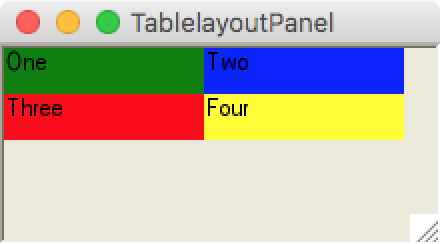
\includegraphics[width=0.45\textwidth]{simpleFlowLayoutPanel1}}
%   \subfigure[]{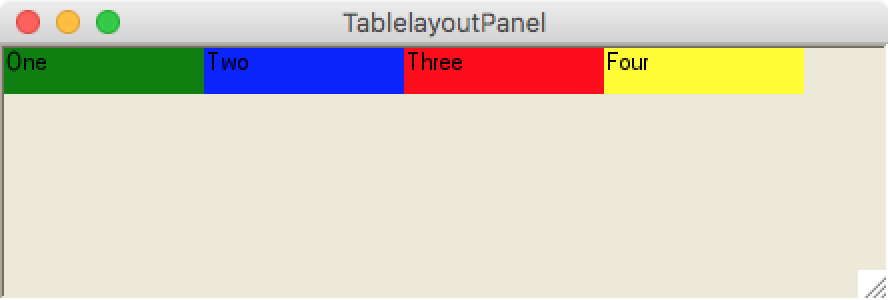
\includegraphics[width=0.9\textwidth]{simpleFlowLayoutPanel2}}
%   \subfigure[]{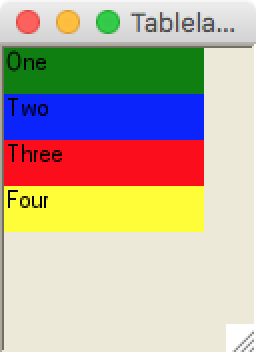
\includegraphics[width=0.225\textwidth]{simpleFlowLayoutPanel3}}
%   \caption{See \Cref{winforms/simpleFlowLayoutPanel}.}
%   \label{fig: simpleFlowLayoutPanel}
% \end{figure}

% %
% \fsCode{winforms/simpleTableLayoutPanel}{winforms/simpleTableLayoutPanel}{\dots}{}
% %
% \begin{figure}
%   \centering
%   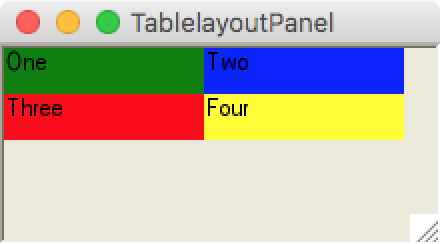
\includegraphics[width=0.4\textwidth]{simpleTableLayoutPanel}
%   \caption{See \Cref{winforms/simpleTableLayoutPanel}.}
%   \label{fig: simpleTableLayoutPanel}
% \end{figure}

% %
% \fsCode{winforms/bounds}{winforms/bounds}{\dots}{}
% %
% \begin{figure}
%   \centering
%   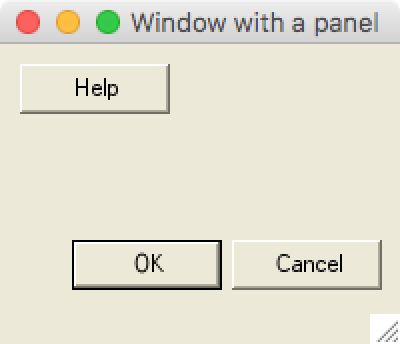
\includegraphics[width=0.3\textwidth]{bounds}
%   \caption{See \Cref{winforms/bounds}.}
%   \label{fig:bounds}
% \end{figure}

% %
% \fsCode{winforms/tabControl}{winforms/tabControl}{\dots}{}
% %
% \begin{figure}
%   \centering
%   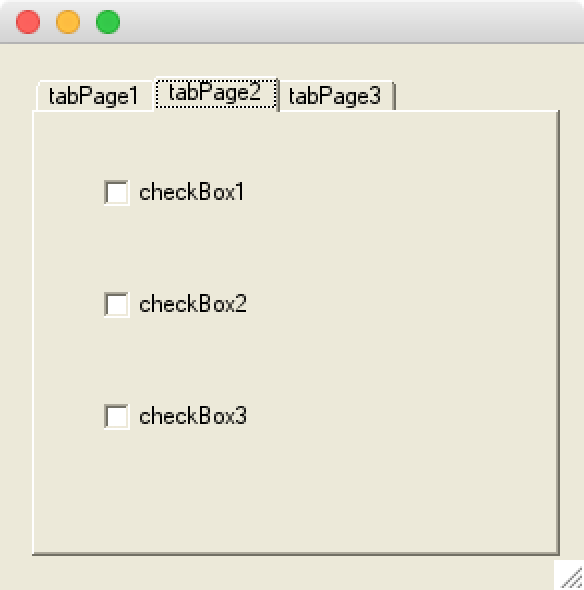
\includegraphics[width=0.3\textwidth]{tabControl}
%   \caption{See \Cref{winforms/tabControl}.}
%   \label{fig: tabControl}
% \end{figure}

% %
% \fsCode{winforms/trackBar}{winforms/trackBar}{\dots}{}
% %
% \begin{figure}
%   \centering
%   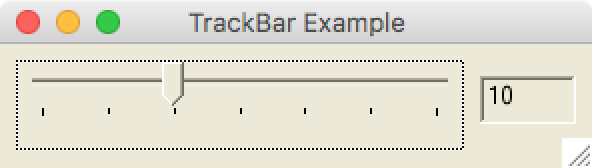
\includegraphics[width=0.3\textwidth]{trackBar}
%   \caption{See \Cref{winforms/trackBar}.}
%   \label{fig: trackBar}
% \end{figure}

% %
% \fsCode{winforms/progressBar}{winforms/progressBar}{\dots}{}
% %
% \begin{figure}
%   \centering
%   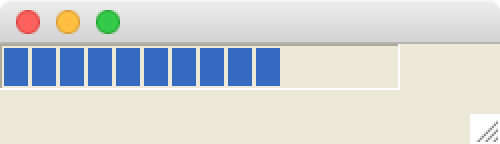
\includegraphics[width=0.3\textwidth]{progressBar}
%   \caption{See \Cref{winforms/progressBar}.}
%   \label{fig:progressBar}
% \end{figure}

% %
% \fsCode{winforms/pixels}{winforms/pixels}{\dots}{}
% %
% \begin{figure}
%   \centering
%   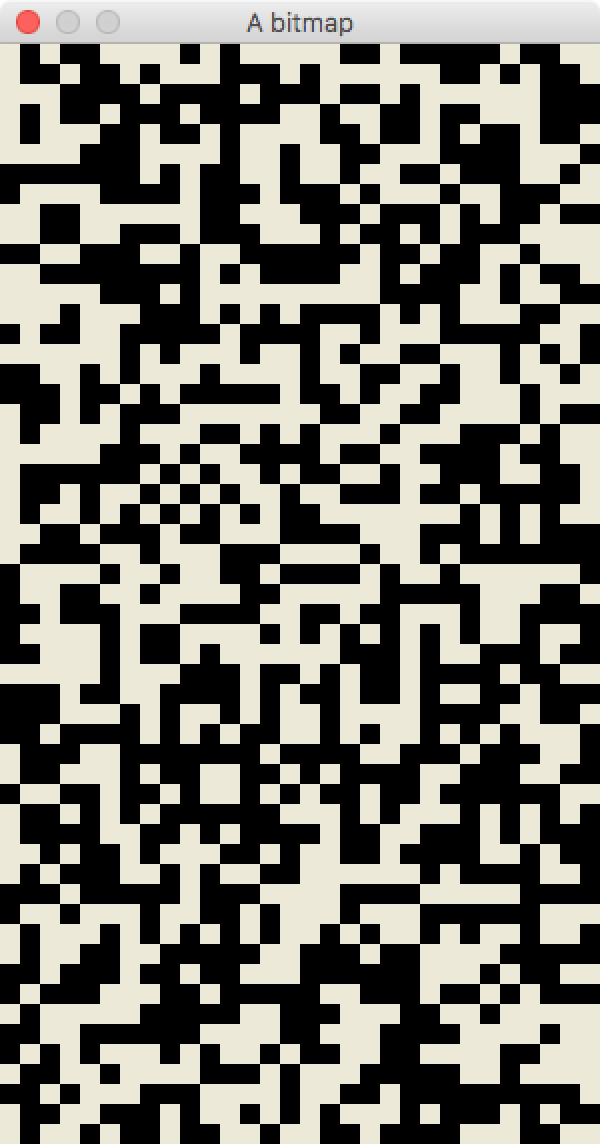
\includegraphics[width=0.3\textwidth]{pixels}
%   \caption{See \Cref{winforms/pixels}.}
%   \label{fig:pixels}
% \end{figure}

% %
% \fsCode{winforms/imageProcessing}{winforms/imageProcessing}{\dots}{}
% %
% \begin{figure}
%   \centering
%   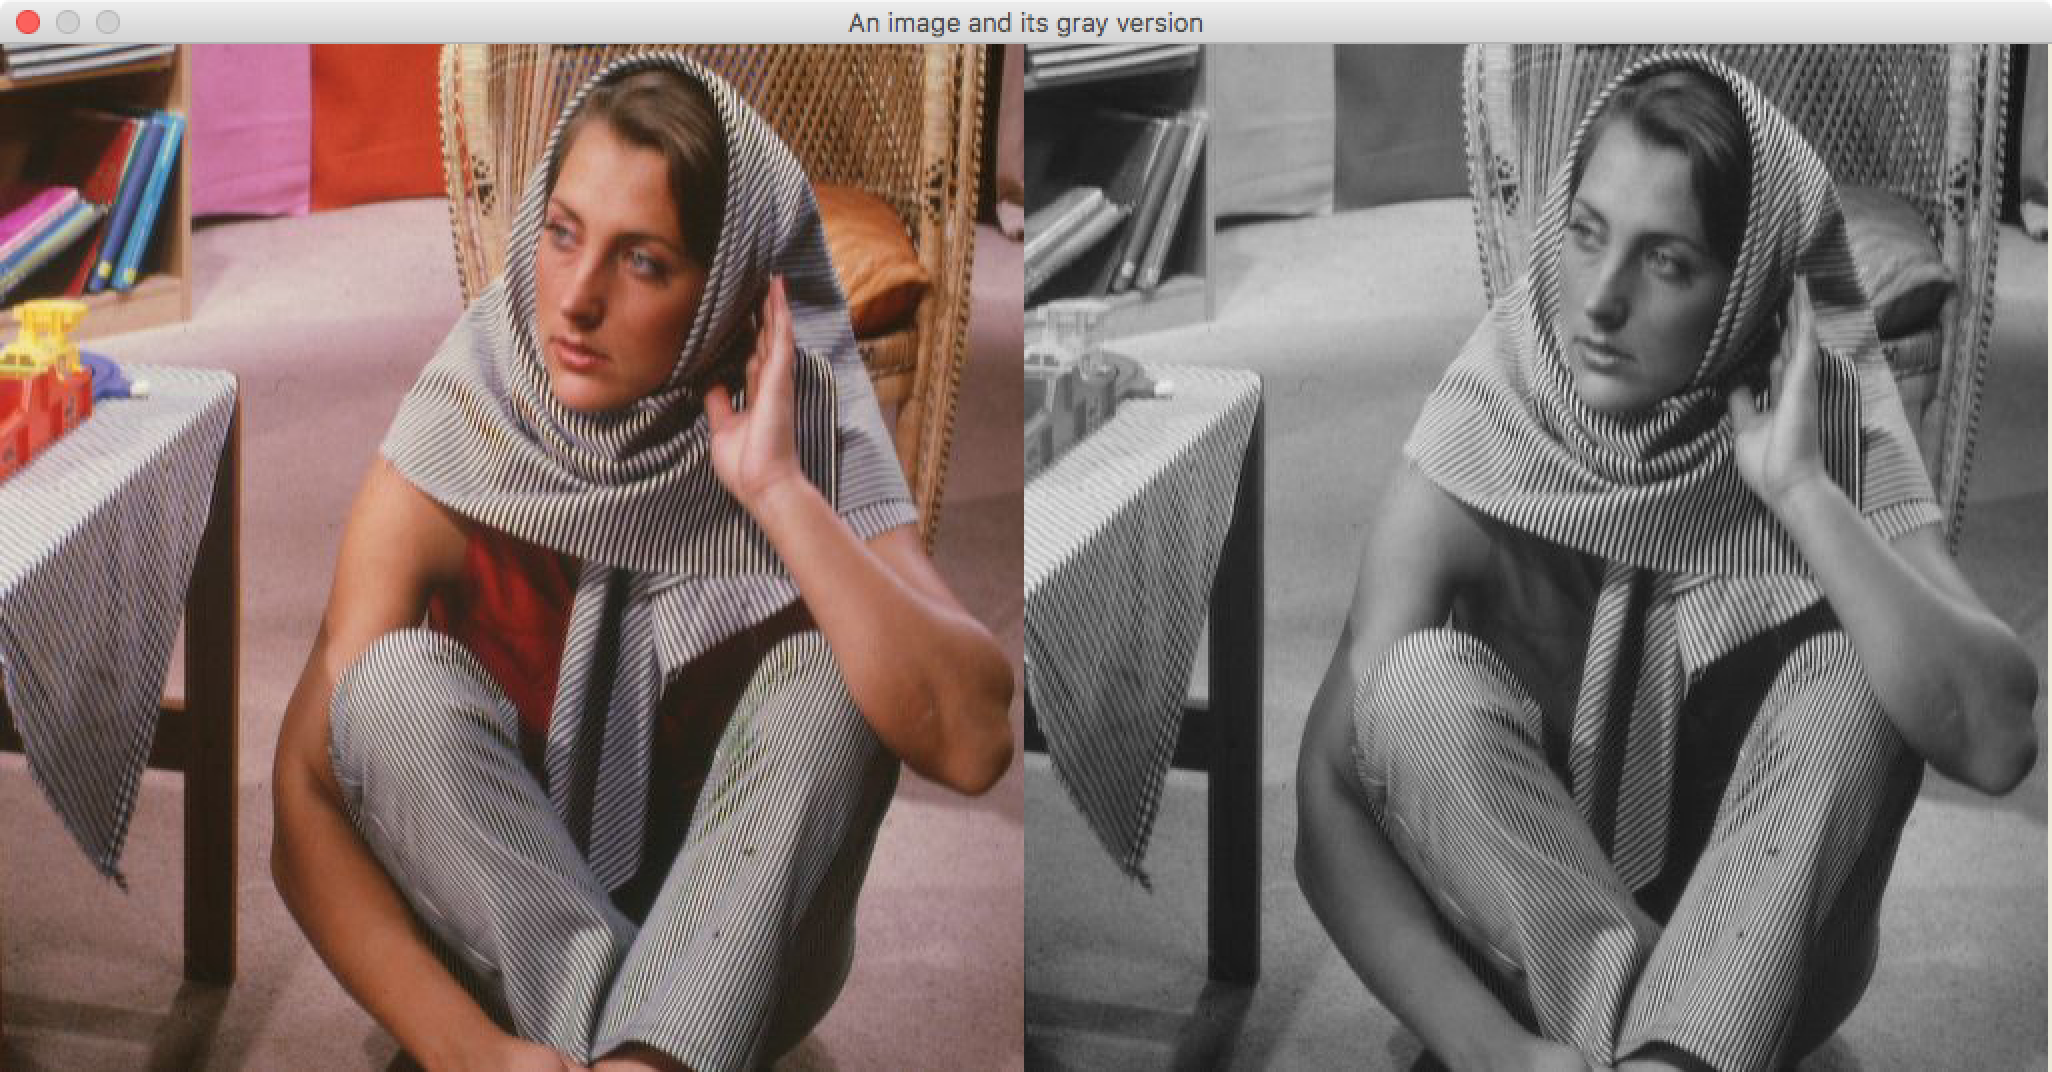
\includegraphics[width=0.3\textwidth]{imageProcessing}
%   \caption{See \Cref{winforms/imageProcessing}.}
%   \label{fig:imageProcessing}
% \end{figure}
% %
% \fsCode{winforms/imageProcessing2}{winforms/imageProcessing2}{\dots}{}
% %
% \begin{figure}
%   \centering
%   \subfigure[]{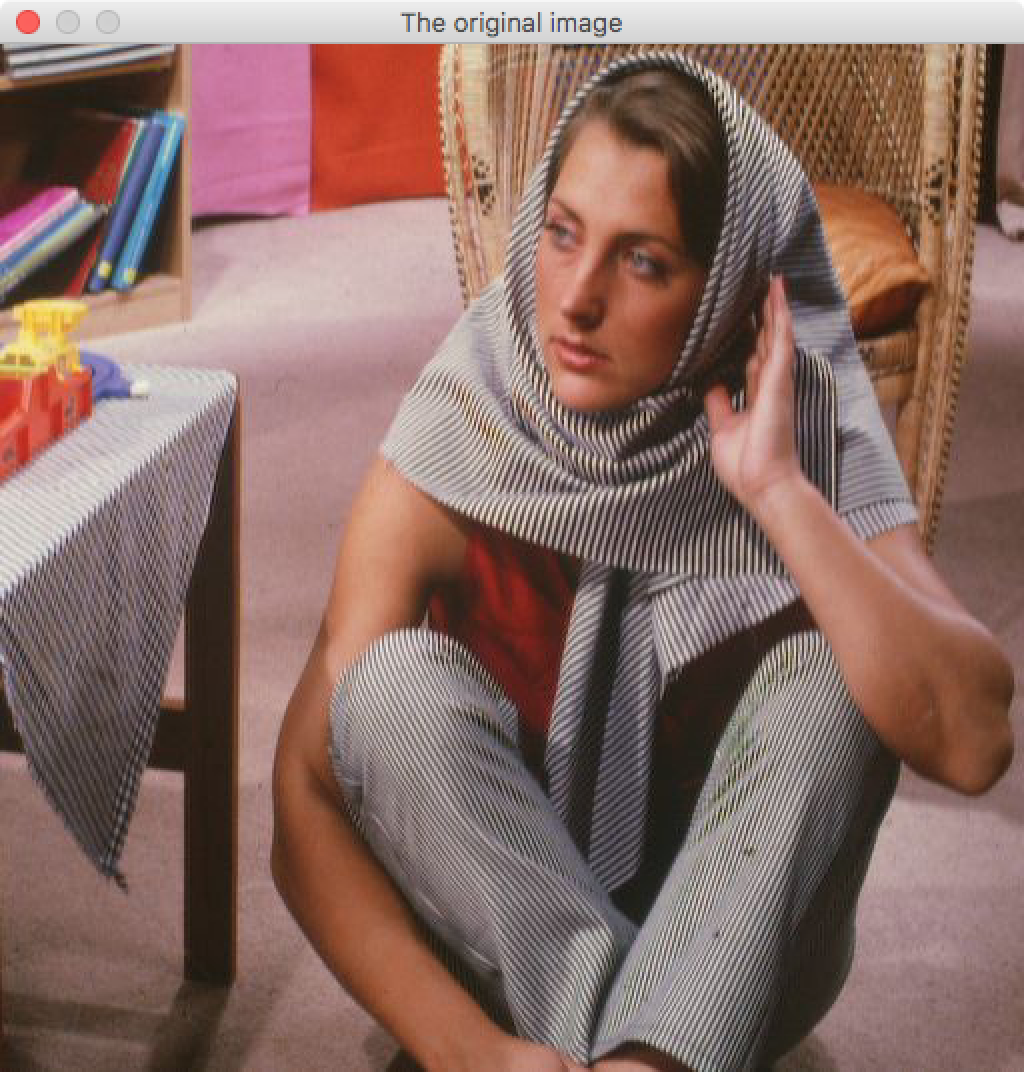
\includegraphics[width=0.3\textwidth]{imageProcessing2_1}}
%   \subfigure[]{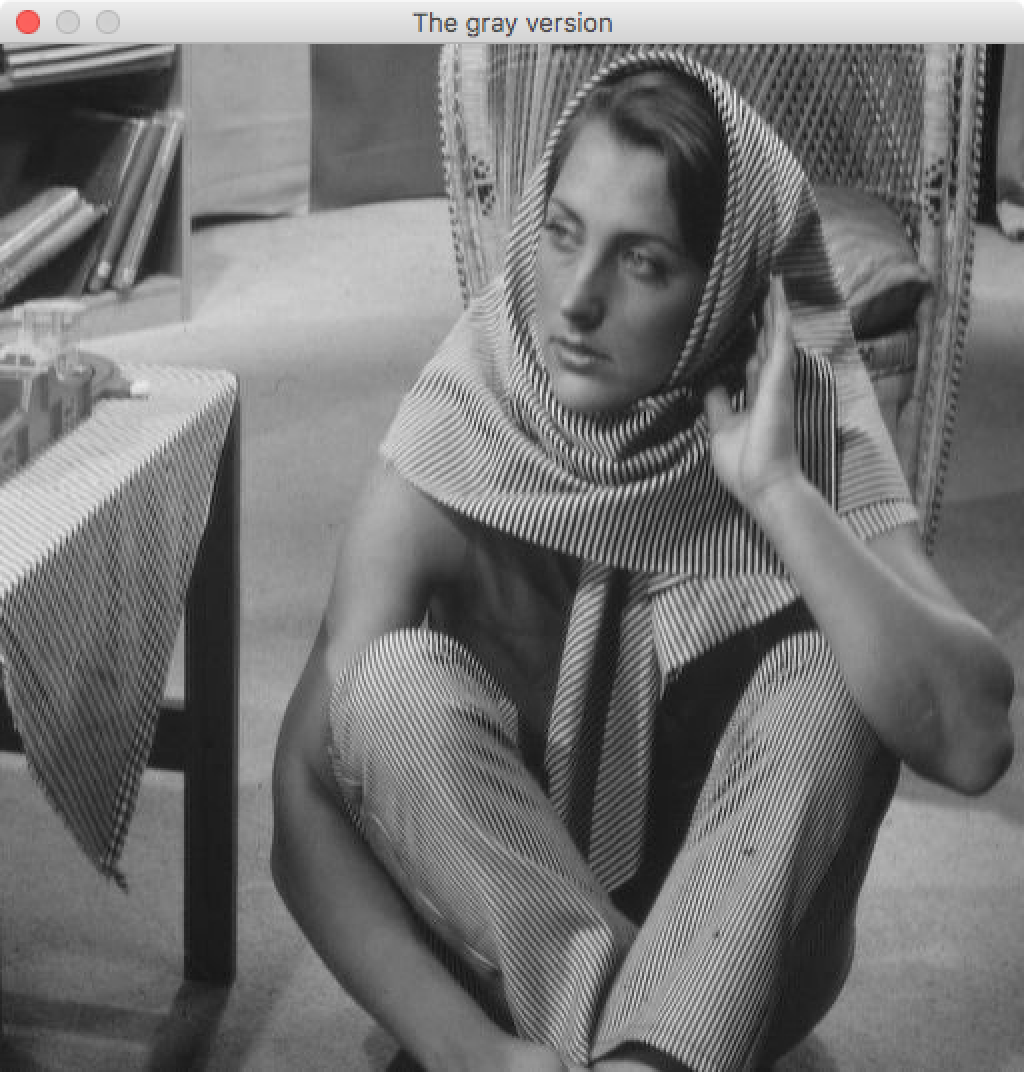
\includegraphics[width=0.3\textwidth]{imageProcessing2_2}}
%   \subfigure[]{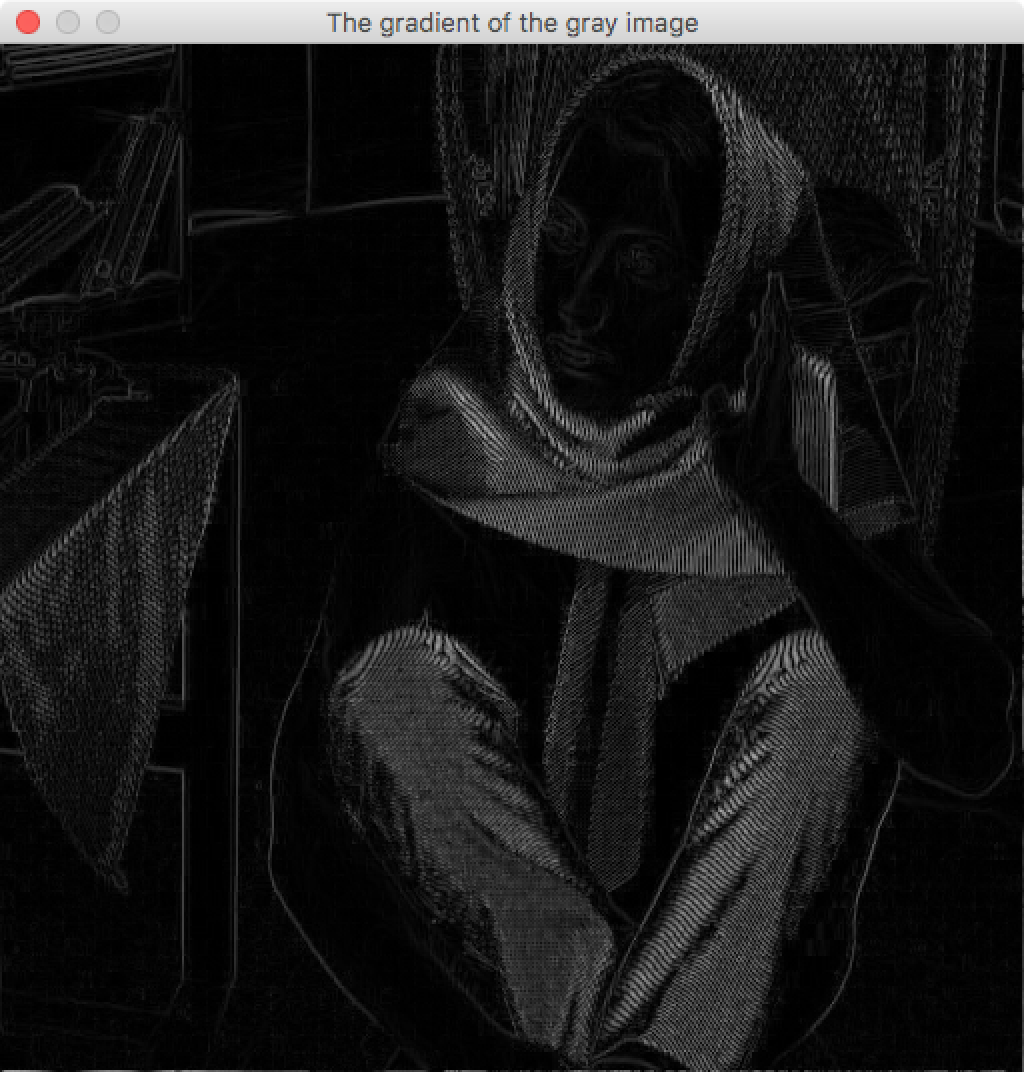
\includegraphics[width=0.3\textwidth]{imageProcessing2_3}}
%   \subfigure[]{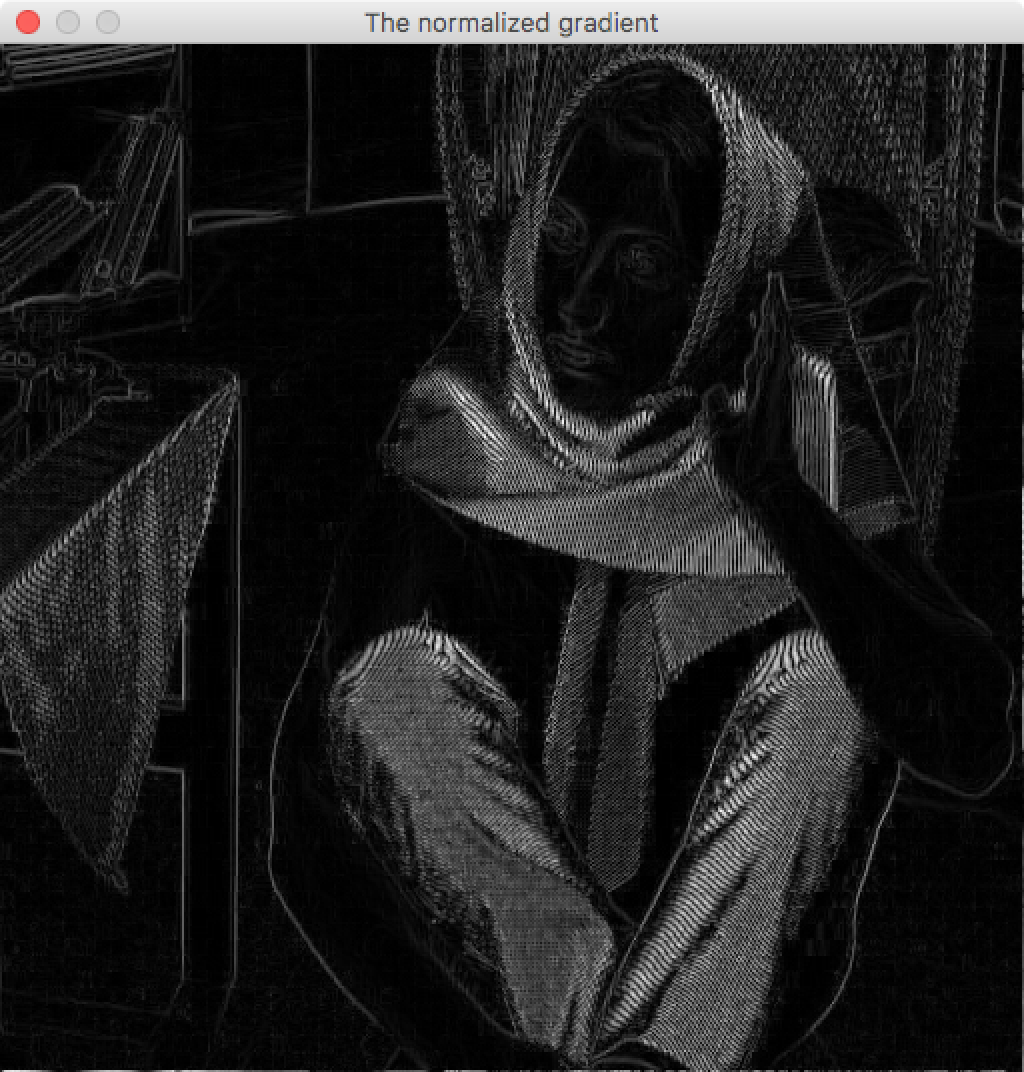
\includegraphics[width=0.3\textwidth]{imageProcessing2_4}}
%   \subfigure[]{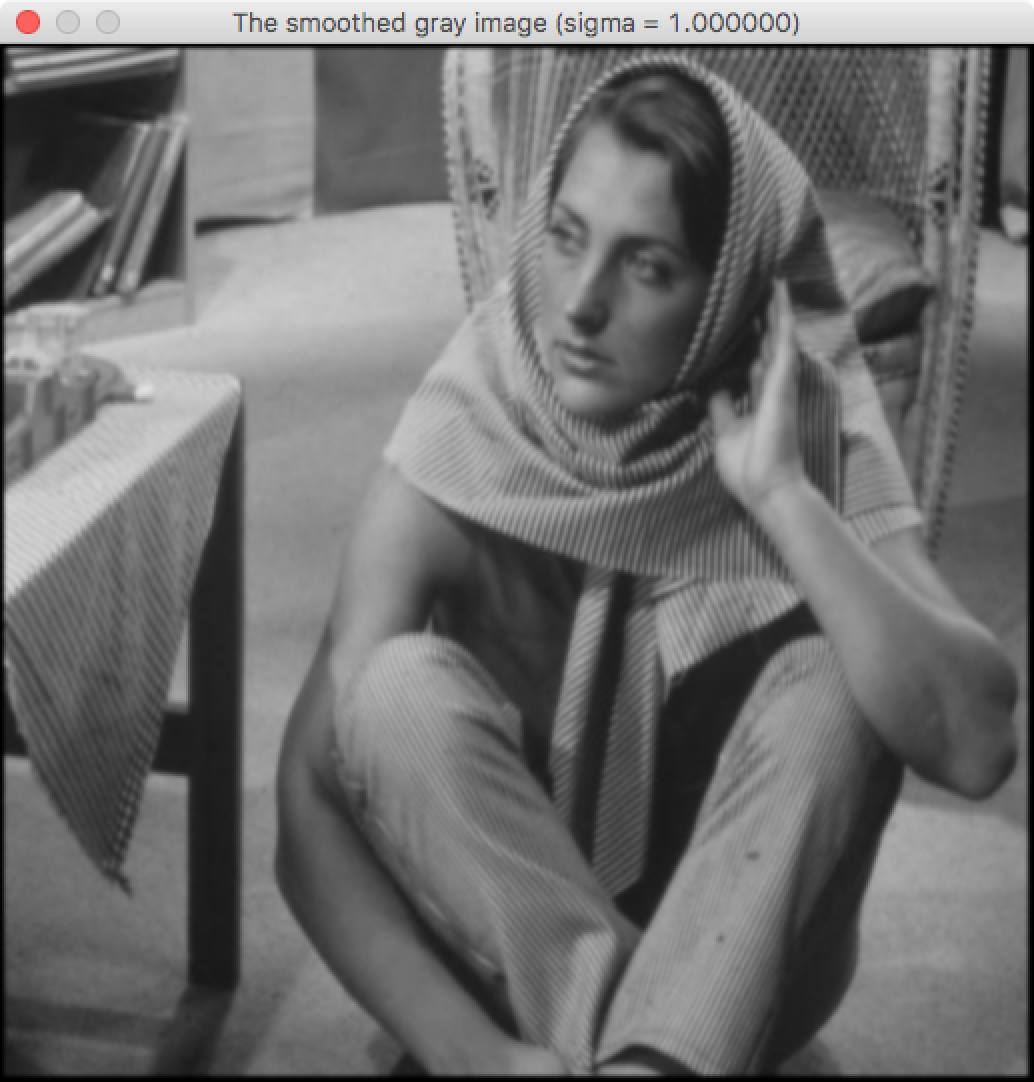
\includegraphics[width=0.3\textwidth]{imageProcessing2_5}}
%   \subfigure[]{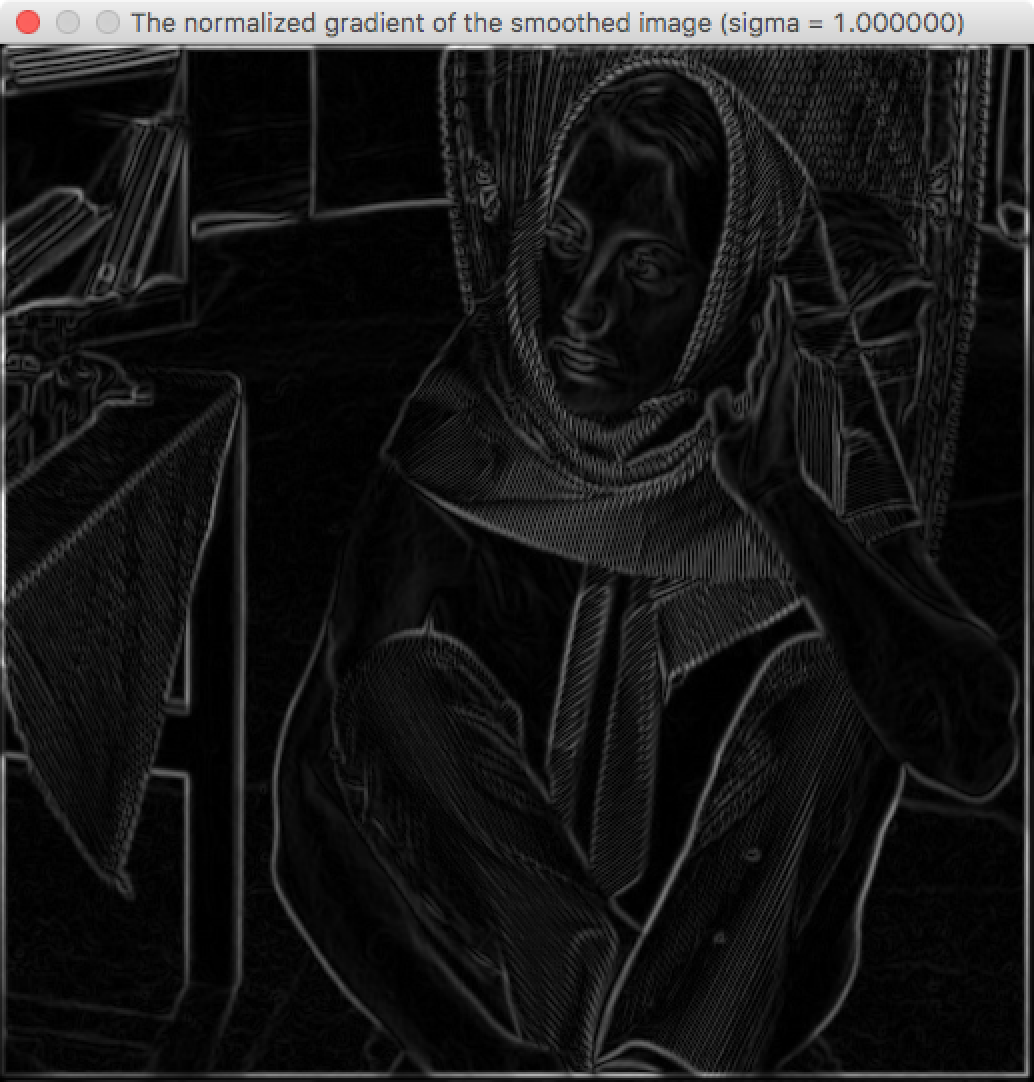
\includegraphics[width=0.3\textwidth]{imageProcessing2_6}}
%   \subfigure[]{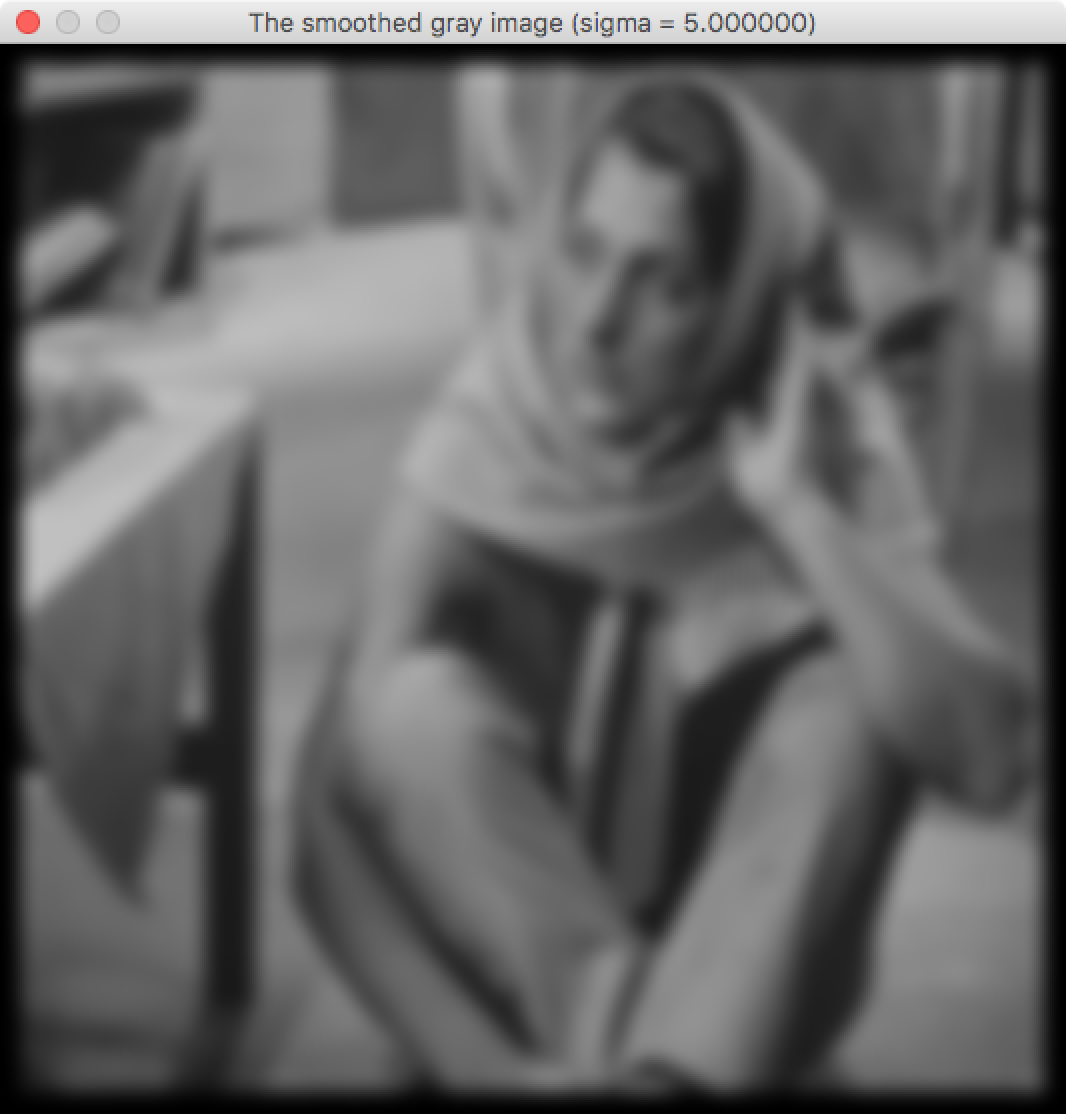
\includegraphics[width=0.3\textwidth]{imageProcessing2_7}}
%   \subfigure[]{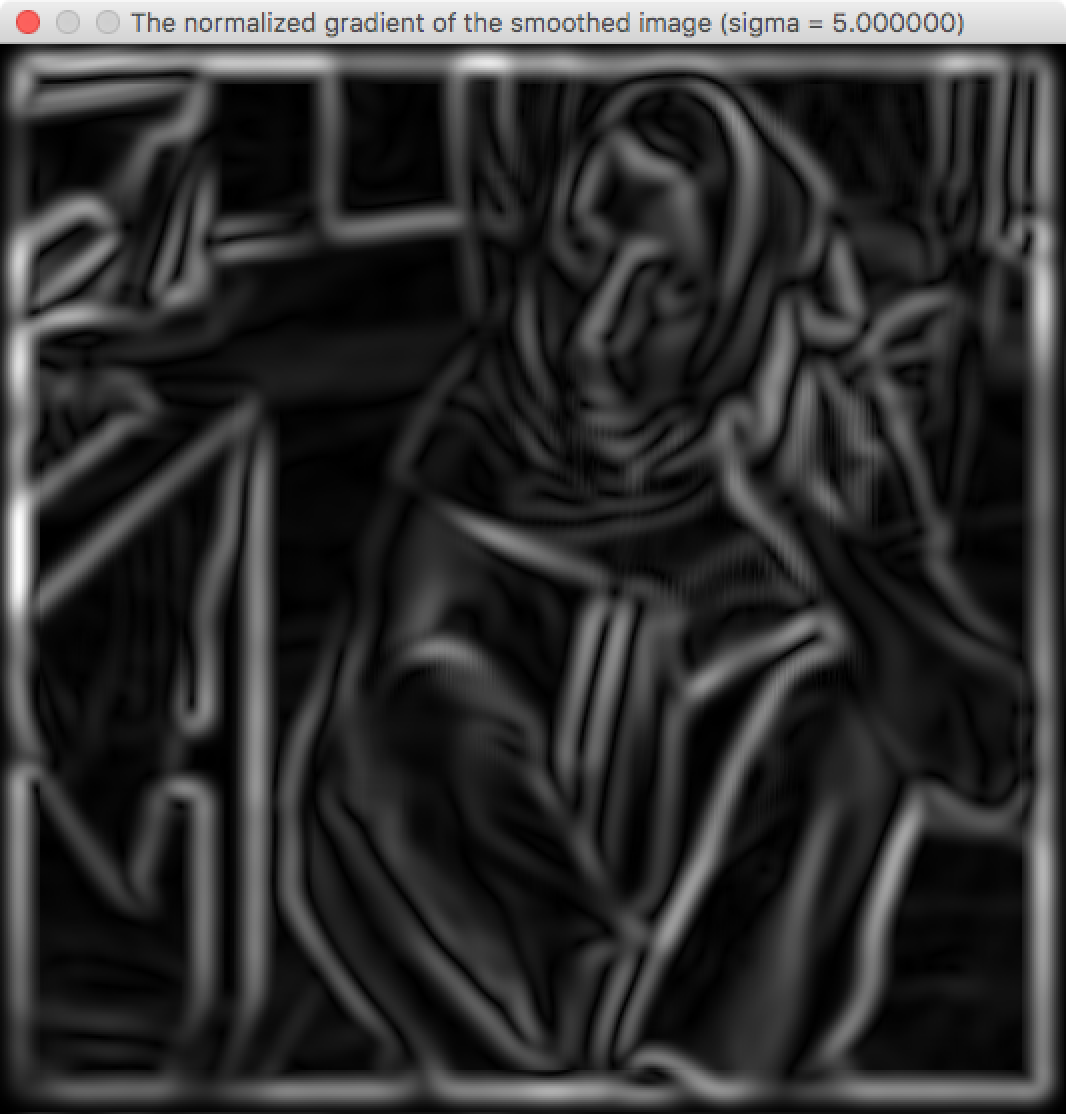
\includegraphics[width=0.3\textwidth]{imageProcessing2_8}}
%   \caption{See \Cref{winforms/imageProcessing2}.}
%   \label{fig:imageProcessing2}
% \end{figure}
\end{document}
